\documentclass[10pt,b5paper,oneside,openright]{book}
\usepackage{config}

\addbibresource{bib/bibliography.bib}

\makeglossaries

\newacronym{admire}{AdMiRe}{Advanced Mixed Realities}

\newacronym{ntnu}{NTNU}{Norwegian University of Science and Technology}
\newacronym{epfl}{EPFL}{Swiss Federal Institute of Technology in Lausanne}
\newacronym{upf}{UPF}{Universidad Pompeu Fabra}
\newacronym{nrk}{NRK}{Norsk Rikskringkasting}
\newacronym{tvr}{TVR}{Romanian Television Society}
\newacronym{csic}{CSIC}{Spanish National Research Council}

\newacronym{iou}{IoU}{Intersection over Union}
\newacronym{dc}{DC}{Dice Coefficient}
\newacronym{pa}{PA}{Pixel\ Accuracy}

\newacronym{tp}{TP}{True Positive}
\newacronym{tn}{TN}{True Negative}
\newacronym{fp}{FP}{False Positive}
\newacronym{fn}{FN}{False Negative}
\newacronym{fpn}{FPN}{False Positive and Negative}


\newacronym{mlbfe}{MLBFE}{Machine Learning Based Foreground Extraction}

\newacronym{ssim}{MS-SSIM}{Multi Scale Structural Similarity Index Measure} 


\begin{document}
\frontmatter
\pagestyle{plain}
\begingroup
\let\cleardoublepage\clearpage
%!TEX root = ../Thesis.tex
\chapter*{\englishabstractname}
\addcontentsline{toc}{chapter}{\englishabstractname}
%
%
\clearpage

%!TEX root = ../Thesis.tex
\chapter*{\norwegianabstractname}
\addcontentsline{toc}{chapter}{\norwegianabstractname}
%
%
\clearpage

\tableofcontents \clearpage
\listoftables    \clearpage
\listoffigures   \clearpage
% \listoftodos     \clearpage
\endgroup

\printglossary[type=\acronymtype] % Print acronyms


\mainmatter
\pagestyle{headings}
%!TEX root = ../Thesis.tex
\chapter{Introduction}\label{cha:introduction}
%
\textcolor{red}{The introduction of the thesis should take the reader all the way from the big picture and context of the project to the concrete task that has been solved in the thesis. In the review part, the background of the project is covered. This leads up to your claim, which is typically that some entity (software, device) or knowledge (research questions) is missing and sorely needed. The agenda part briefly summarises how your thesis contributes. The \emph{agenda} part should inform the reader about the structure of the rest of the document, since this may vary significantly between theses.}

%!TEX root = ../Thesis.tex
\chapter{Background}\label{cha:background}
%
\textcolor{red}{Research projects should always be based on previous research on the same and/or related topics. This should be described as a background to the thesis with adequate bibliographical references. If the material needed is too voluminous to fit nicely in the review part of the introduction, it can be presented in a separate background chapter.}


\section{Motivation}\label{sec:motivation}

The last decades traditional television viewing numbers have steadily been declining \cite{ssb_seertall}. People do not find TV as appealing as they once did. Today, more people seem to find more engaging and personal forms of entertainment elsewhere. Currently, the only form of doing, what one could call an engaging TV broadcast, is through the use of social media and hybrid broadcast broadband TV by incorporating comments, videos and audio from the audience into the TV broadcast. Sadly, this form of engagement is quite limited and does not give proficient results. 

\section{AdMiRe}\label{sec:admire}
Wanting to innovate and create better experiences in this space, the AdMiRe \cite{admire} (Advanced Mixed Realities) project has been formed as a collaboration between Brainstorm, Disguise, NTNU, EPFL, UPF, NRK, Premiere, TVR and CSIC. The aim of the AdMiRe project is to use mixed reality solutions to enable audiences at home to be incorporated into live TV programs and interact with the other people in the TV studio. 

Doing this using the available technology is hard because of the technical challenges. To make this easier AdMiRe is set out to develop and simplify key modules. 

\begin{figure}[H]
  \centering
  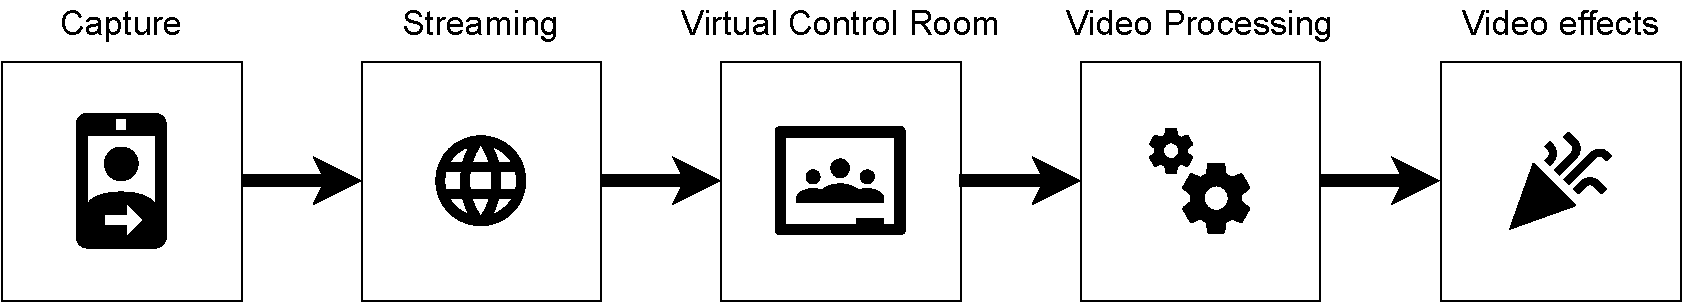
\includegraphics[width=0.9\textwidth]{img/admire_system.pdf}
  \caption{AdMiRe system flow}
  \label{fig:admire_system}
\end{figure}


An important aspect of this technology is to make it look like the participant is in the studio, and to make it look like the participant is in the studio, the participant has to be extracted out of its own environment and inserted naturally into the studio environment. That's why we will take a look at the machine learning silhouette extraction module currently used in the AdMiRe project. We will try to evaluate the quality of experience and generally assess the quality of the technology by running some subjective and objective tests on the silhouette extraction and see if there is any correlation between them. 


\subsection{\acrlong{mlbfe}}\label{sec:mlbfe}
The AdMiRe project is using a \acrlong{mlbfe} algorithm which has been developed by the multimedia signal processing group of EPFL. 

The algorithm is MobileNet-UNet constellation. This constellation is constructed of a U-Net based autoencoder, where the encoder part has been replaced with a MobileNetV2 architecture. 

\subsubsection{U-Net}\label{sec:unet}
A U-Net architecture is a pipeline of compressions, using pooling layers, and decompressions, using transposed convolution layers \cite{ronneberger2015unet}. \autoref{fig:unet} gives a simplified 3-level illustration of this architecture. The pooling layers are used to reduce the dimensionality of the input, while the transposed convolution layers will increase the dimensionality. Each layer also gives a skip connection to the matching output layer for information retention. Information from each level contributes to the final reconstruction where convolution layers merge the final information. One of the highlights of this architecture is the low loss function.  

\begin{figure}[H]
  \centering
  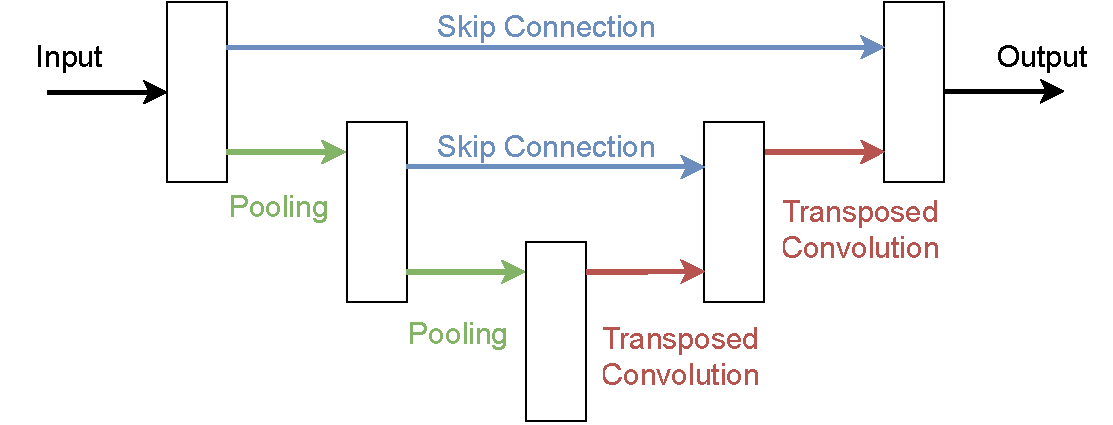
\includegraphics[width=0.9\textwidth]{img/ML/unet.pdf}
  \caption{Simplified U-Net architecture. }
  \label{fig:unet}
\end{figure}

\subsubsection{MobileNetV2}\label{sec:mobilnet}
MobileNetV2 is an improvement \cite{sandler2019mobilenetv2} of the original MobileNet \cite{howard2017mobilenets}. MobileNet is a lightweight architecture suitable for low computational power use cases using depth-wise separable convolution. 

MobileNetV2 was introduced to improve the performance. It did this by including some changes to the structure of the convolution layers with the introduced a point wise convolution layer with a linearity to the beginning of the layers \cite{vision_based}. Each layer also has a ReLU and a residual bottleneck connection is used to reduce the input size. ReLUs, Rectified Linear Units, is an  activation function which is zero in the negative dimension, but linear in the positive. A simplified illustration of the architecture of the MobileNetV2 model can be found in \autoref{fig:mobnetv2}.

\begin{figure}[H]
  \centering
  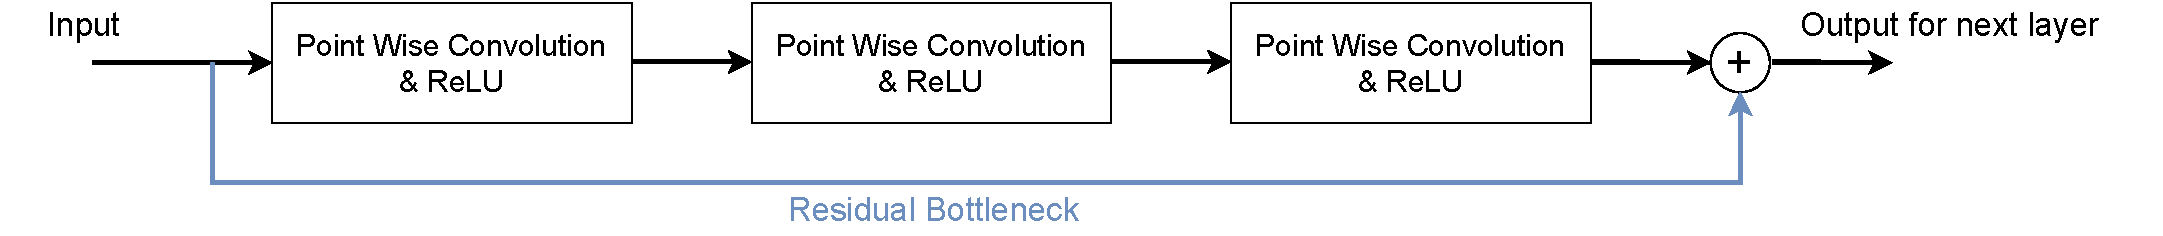
\includegraphics[width=1\textwidth]{img/ML/MobileNetV2.pdf}
  \caption{Simplified MobileNetV2 architecture. }
  \label{fig:mobnetv2}
\end{figure}

\subsubsection{MobileNet-UNet}\label{sec:mobilenet-unet}
With the combination of the two methods discussed in \autoref{sec:unet} and \autoref{sec:mobilnet}, one gets a architecture which decodes up-sampled features using transposed convolution layers with corresponding down-sampling stages \cite{8575250}. Each layer gets fused with it's corresponding layer with an element-wise addition. A simplified version of the architecture is illustrated in \autoref{fig:mobilenet-unet}. 

\begin{figure}[H]
  \centering
  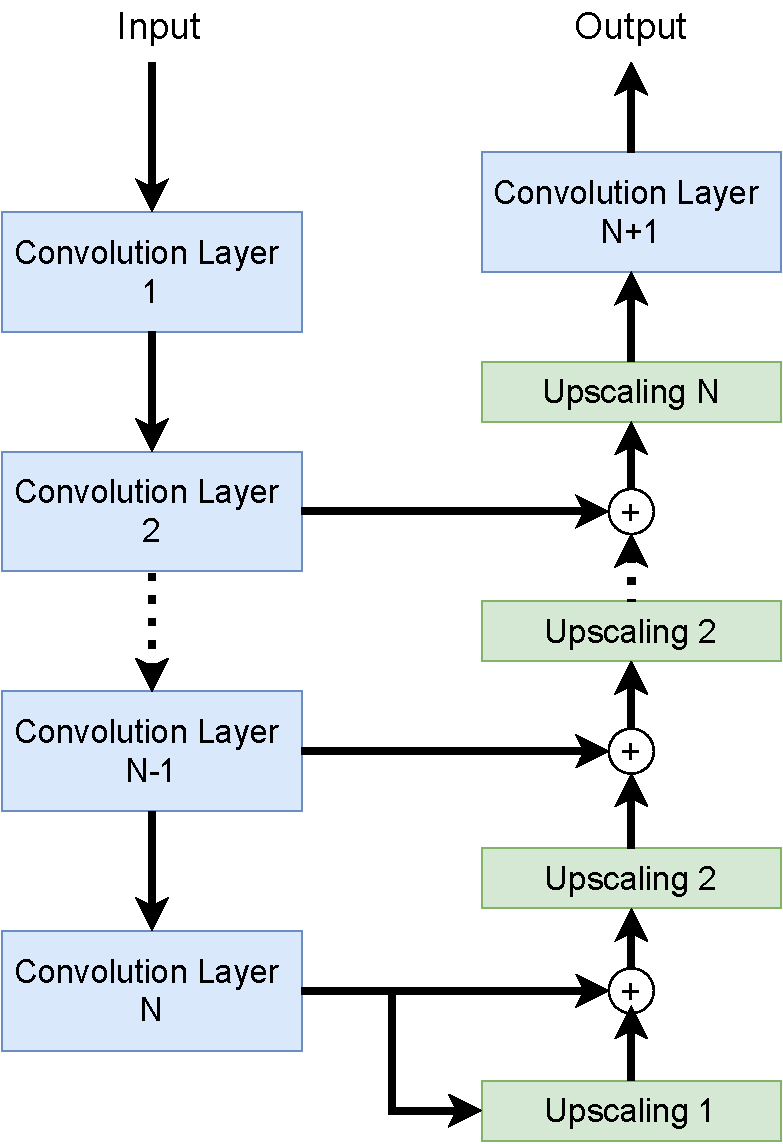
\includegraphics[width=.4\textwidth]{img/ML/MobileNet-UNet.pdf}
  \caption{Simplified MobileNet-UNet architecture. }
  \label{fig:mobilenet-unet}
\end{figure}

\subsubsection{Training, validation and testing}\label{sec:training}
The learning architecture of the model is based on the model used in \cite{bmshj2018}, with a optimisation for \acrfull{ssim}. \acrshort{ssim} is a method for predicting the perceived quality of digital signals where degradation is viewed as perceived change in structural information. The Multi Scale version is conducted over multiple samples, with multiple stages of sub-sampling \cite{mssssim}. The architecture is further using the pre-trained models available from TenserFlows Compression \cite{tensorflow_compression}.

The model has been trained, validated and tested with the human segmentation data set presented in \cite{gmnu21}. In this data set, humans have been set as foreground, while the rest of the frame is set as the background. Using this data set, the model has been trained on semantic segmentation of humans with object removal, in this case being the entire background


\section{Previous work}\label{sec:previous}

\textit{Some of the following is taken from \cite{prp} and have been adapted to the fit this report.}
\subsection{Quality of Experience}
\label{sec:qoe}
QUALINET white papers defines Quality of Experience as following \cite{book_QoE}

\begin{quote}
The degree of delight or annoyance of the user of an application or service. It results from the fulfilment of his or her expectations with respect to the utility and/or enjoyment of the application or service in the light of the user’s personality and current state.
\end{quote}

Quality of Experience is a field which is based on multiple disciplines such as social psychology, cognitive science, economics and engineering service with a focus on understanding overall human quality requirements.

There are a number of influencing factors in regards of the general Quality of Experience, namely human, system and contextual influencing factors \cite{factors_QoE}.
\begin{itemize}
    \item \textbf{Human influencing factors} (HIF) can be divided into two parts — low level and high level. Low level factors are factors such as age, physical form, emotions and mental constitution, while high level are factors such as previous knowledge regarding the matter. 
    \item \textbf{System influencing factors} (SIF) which is the technical elements in role. The type of content being consumed, what kind of media (meaning factors such as encoding, resolution, sample rate), network constrains (e.g. bandwidth, delay and jitter) and device differences (e.g. different screen sizes, resolutions, frame rate and audio quality)
    \item \textbf{Context influencing factors} (CIF) are the surrounding factors which affects the user. The physical location (e.g. lighting and surrounding space), social relationships (e.g. inter-personal relationships), type of task, interruptions, time of day, how many times the user has been using these type of systems before and more technical contextual challenges (e.g. a system which has to work together with other separate systems) are all influencing aspects.
\end{itemize}


\subsection{Semantic Segmentation}
When doing semantic segmentation, we mean assigning each pixels in an image a semantic class label \cite{csurka2013good}. Semantic segmentation has several use cases, such as scene understanding, object removal and local class based image enhancement. The different use cases require different level of segmentation, because of their complexity. Scene understanding might need a rougher segmentation, than what object removal might need. This makes semantic segmentation difficult to evaluate. What makes a good segmentation is entirely up to the use case and the success of the segmentation is measured by the success of the end application \cite{csurka2013good}.


\subsection{Subjective Measurement}
\label{sec:measurement}
In a use case where we want to extract the silhouette of a human to be inserted into another setting, the overall quality of the video can be strongly subjective. Since a silhouette extraction can be prone to seemingly random cuts and jitter, the perceived quality of the video from a human perspective can be strongly compromised even though objective quality measures gives a strong measure. 

\subsubsection{Mean Opinion Score and Likert Scale}
\label{sec:mos}
The Mean Opinion Score (MOS) \cite{Streijl2016} and Likert scale \cite{likert_scale} is widely used measurement for media signals and quality. This  measure is often represented as a 5-point answer system, represented in \autoref{tab:rating_label}. While these are popular methods, the usefulness is often debated due to inherent limitations of measurements in a single scalar value \cite{wiki_mos}. 

The subjective quality evaluation requires a lot of human resources and can be time consuming. The mean opinion score method is otherwise prone to misuse or misinterpretation, as the design of the subjective experiments have an important influence. The objective media quality metrics do also rely on data from the subjective experiments for tuning and validation, and it can therefore be challenging to make meaningful measurements and interpret the resulting findings correctly \cite{Streijl2016}.


\begin{table}[]
    \centering
    \begin{tabular}{ |c|c|c|c|c|c| } 
         \hline
         \textbf{Rating} & 1 & 2 & 3 & 4 & 5 \\
         \hline
         \textbf{Label} & Bad & Poor & Fair & Good & Excellent \\ 
         \hline
    \end{tabular}
    \caption{Rating and labels for subjective answers}
    \label{tab:rating_label}
\end{table}

\subsection{Objective measurement}\label{sec:objective_measurement}
Objective measurements are pixel wise comparisons of the pixels in the resulting images, up against a given truth table. The coming sections present some of the most popular measures. 

\subsubsection{\acrlong{pa}}
\acrfull{pa} is a simple measure which takes the number of correctly classified pixels, the number of \acrlong{tp} and \acrlong{tn}, over the total number of pixels in an image, the number of \acrlong{tp}, \acrlong{tn}, \acrshort{fp} and \acrshort{fn}. Easily said its the percentage of correctly classified pixels in an image \cite{jeremy}.

\begin{equation}
    \acrlong{pa} = \frac{\acrshort{tp}+\acrshort{tn}}{\acrshort{tp}+\acrshort{tn}+\acrshort{fp}+\acrshort{fn}}
\end{equation}

While this is a simple and effective measurement, it is prone to class imbalance \cite{tiu}. This can lead to a high score even though the classification itself is bad. \autoref{fig:pa} highlights this problem. The ground truth to the left has a white section in the middle, but the classifier has been unable to classify this area correctly. Since the white area in the ground truth only covers 1\% of the image, we get a 99\% pixel accuracy even though the classifier has completely failed to classify the segment.

\begin{figure}[H]
  \centering
  
\includegraphics[width=0.9\textwidth]{img/objective_measures/pa.pdf}
  \caption{Truth table to the left, and classified results to the right}
  \label{fig:pa}
\end{figure}

\subsubsection{\acrlong{iou}}
\acrfull{iou}, also known as the Jaccard index originally developed by Paul Jaccard \cite{jaccard}, has become the standard performance measure of image semantic segmentation\cite{Rezatofighi_2019_CVPR}. The measure outputs a percentage of overlap between the predicted region and the ground truth of a image segmentation. This is a count based measure looking at the intersection of the predicted and the ground truth over the union of the predicted area and ground truth. If we have a binary classification problem, we can use the number of \acrlong{tp} over the number of \acrlong{fp}, \acrlong{fn} and \acrlong{tp}.
\cite{10.1007/978-3-319-50835-1_22}

\begin{equation}
    IoU = \frac{intersection}{union} = \frac{|target \cap prediction|}{|target \cup prediction|} = \frac{\acrshort{tp}}{\acrshort{fp} + \acrshort{fn} + \acrshort{tp}}
\end{equation}


\begin{figure}[H]
  \centering
  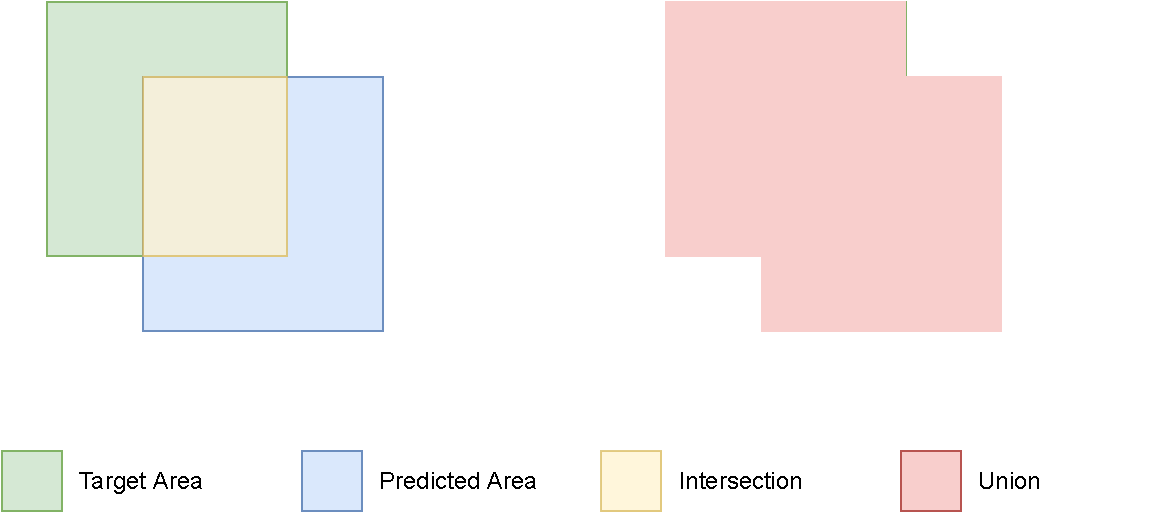
\includegraphics[width=0.9\textwidth]{img/objective_measures/iou.pdf}
  \caption{Intersection over Union}
  \label{fig:iou}
\end{figure}

\subsubsection{\acrlong{dc}}
The \acrfull{dc} is a similar metric to \acrlong{iou}. Like \acrlong{iou}, \acrlong{dc} is a statistic used to measure the similarity between two samples \cite{sorensen}\cite{dice}. The measure outputs a percentage between two times the overlap and the total number of pixels in both images, as seen in \autoref{eq:dc} and illustrated in \autoref{fig:dc}. For a binary classification the measure outputs a percentage of two times the number of \acrlong{tp} and the total of two times the \acrlong{tp}, \acrlong{fp} and \acrlong{fn}.

\begin{equation}\label{eq:dc}
    \acrshort{dc} =  \frac{2|target \cap prediction|}{|target| + |prediction|} = \frac{2\acrshort{tp}}{2\acrshort{tp}+ \acrshort{fp} + \acrshort{fn}}
\end{equation}

\acrlong{dc} and \acrlong{iou} will always be positively correlated for a fixed ground truth, and will always be within a factor of two of each other, as stated in \autoref{eq:dc_iou_relation}.

\begin{equation}\label{eq:dc_iou_relation}
    \frac{\acrshort{dc}}{2} \leq \acrshort{iou} \leq \acrshort{dc}
\end{equation}

While \acrlong{iou} tends to penalise single instances of bad classification more than the \acrlong{dc}. The \acrlong{dc} works better for measuring the average performance of a parameter. For example, imagine we have two classifiers, A and B. If A were to be a great classifier, but had one bad classification, the average \acrlong{iou} score, would be penalised much harder than the average \acrlong{dc}, since this is not so prone to outlier values. This would result in giving the impression that B might be a better classifier than A, if we were only to look at the \acrlong{iou} \cite{276144}.

\acrlong{dc} \textbf{(S)} being so similar to \acrlong{iou} \textbf{(J)} and can easily be converted using the relations in \autoref{eq:iou-dc} and \autoref{eq:dc-iou} \cite{wiki_dc}.

\begin{minipage}{.45\linewidth}
\begin{equation}\label{eq:iou-dc}
    J = \frac{S}{2 - S}
\end{equation}
\end{minipage}
\begin{minipage}{.45\linewidth}
\begin{equation}\label{eq:dc-iou}
    S = \frac{2J}{1 + J}
\end{equation}
\end{minipage}

\begin{figure}[H]
  \centering
  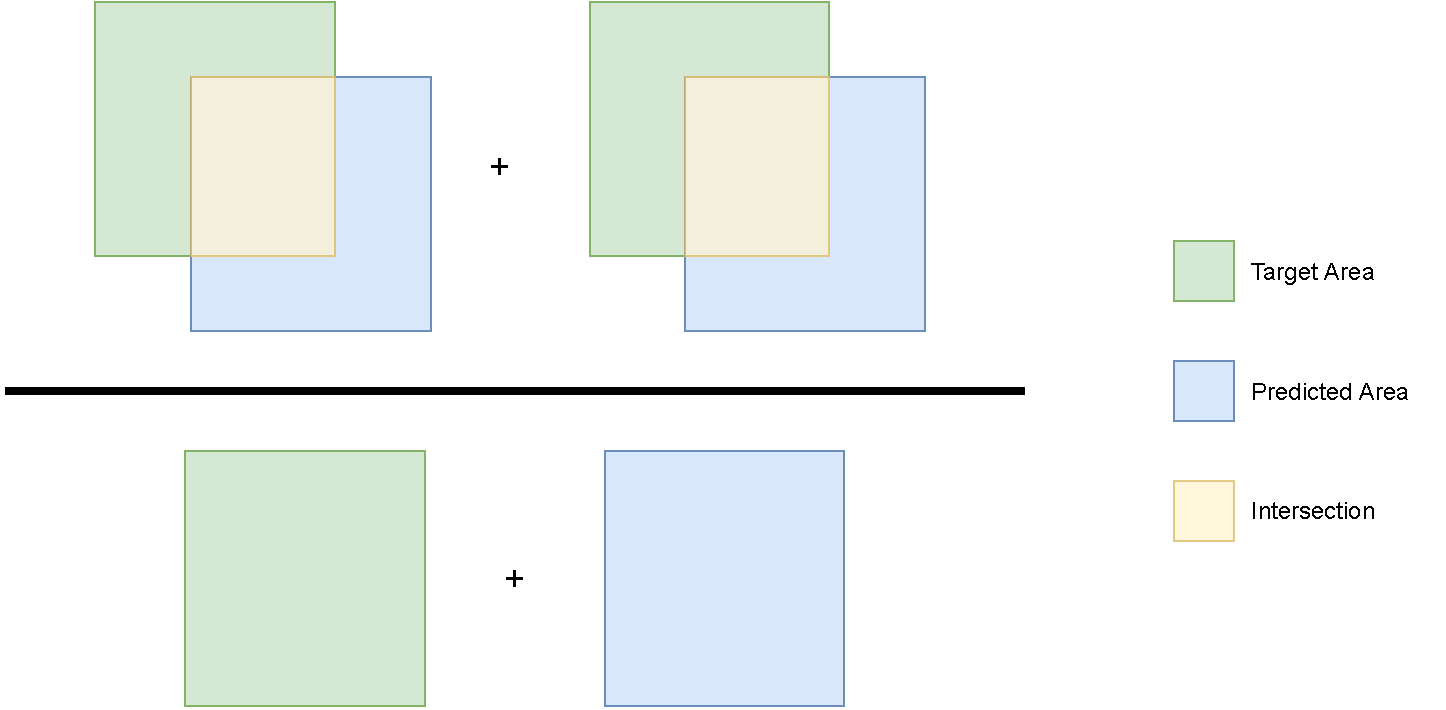
\includegraphics[width=0.9\textwidth]{img/objective_measures/dc.pdf}
  \caption{Dice Coefficient}
  \label{fig:dc}
\end{figure}

%!TEX root = ../Thesis.tex
\chapter{System Design}\label{cha:system_design}
%

\textcolor{red}{The method chapter should describe in detail which activities you undertake to answer the research questions presented in the introduction, and why they were chosen. This includes detailed descriptions of experiments,surveys, computations, data analysis, statistical tests etc.}

We will design a system which will help us answer the following \textbf{research question}:
\begin{tcolorbox}

\begin{displayquote}
    $\mathbf{RQ}$\textbf{:} Is there a correlation between the objective measures pixel accuracy,  and Dice Coefficient and the subjective measures of satisfaction, level of artifacts and level of annoyance in the machine learning based foreground extracted processed videos?
\end{displayquote}

\end{tcolorbox}


To help us investigate the research question, we also form some supporting hypotheses. We expect that the videos which gets a low score on the objective measures, also will receive a poor score subjectively. 
\begin{tcolorbox}
\begin{displayquote}
    $\mathbf{H_1}$\textbf{:} The videos with poor objective statistics will also receive poorer rating from the subjective testing.
\end{displayquote}
\end{tcolorbox}

Another interesting subject, is to see if the videos which received a good objective testing, will be matched with a good rating from the participants

\begin{tcolorbox}
\begin{displayquote}
    $\mathbf{H_2}$\textbf{:} The videos with good objective statistics will also receive a good rating from the subjective testing.
\end{displayquote}
\end{tcolorbox}

In the coming sections we go through how we designed a system which tried to test this. 



\section{Video setup}
We will create a system consisting of several parts. The basic construction will be set of foreground videos in front of a green screen (figure \ref{fig:videos}a), where we try to create situations which we imagine could reflect some real world usage. The resulting video will be edited using chroma key compositing to remove the background (figure \ref{fig:videos}b). Further on, the video will be inserted onto different kind of background videos (figure \ref{fig:videos}c). This video will finally be processed by our machine learning based foreground extractor, which will output our segmented silhouette extraction (figure \ref{fig:videos}d). 

\begin{figure}[H]
  \centering
  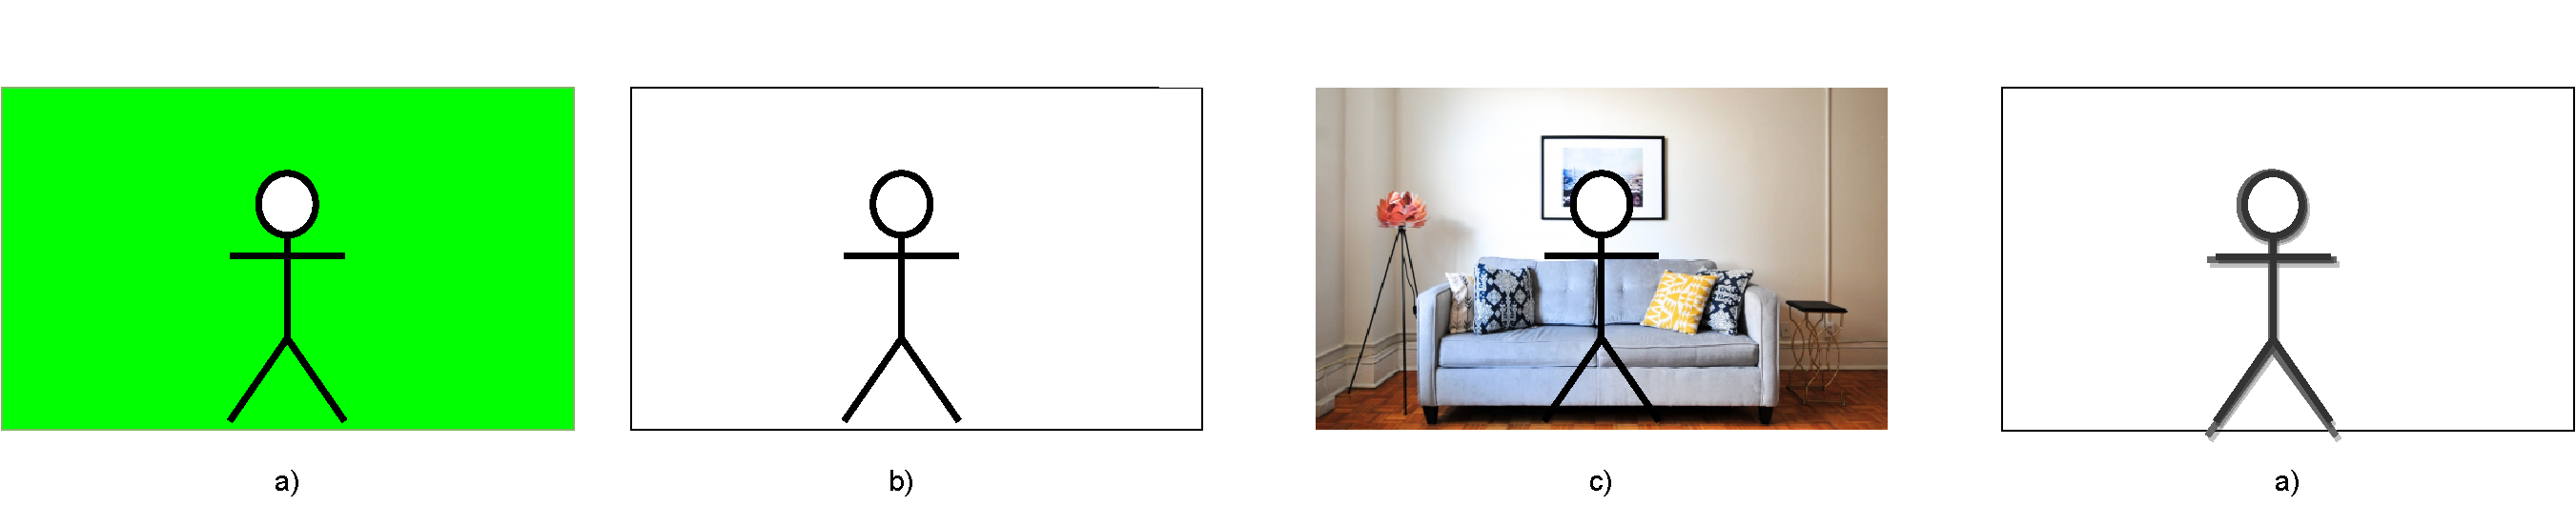
\includegraphics[width=\textwidth]{img/video_setup/video_system_design.pdf}
  \caption{Phases of video system design}
  \label{fig:videos}
\end{figure}

We will create three different backgrounds, described in \autoref{sec:backgrounds}, along with four different type of foreground videos, described in \autoref{sec:foregrounds}. By combining the background and foreground videos we will have a total of twelve (12) videos to run our objective and subjective analysis. Each video will have a duration of ten (10) seconds filmed at 30 fps. This will result in each video having 300 frames.

\subsection{Backgrounds}\label{sec:backgrounds}

An on-site shot of each background shot can be found in \autoref{cha:appendix-backgrounds}. Each of the background shots in the following section has been taken from frame 150 of the 300 frames video.

\subsubsection{Simple white wall}
A simple white wall with typical hall way lighting was selected to try to give the algorithm a ''simple'' task where the foreground would be in stark contrast to the background.

\begin{figure}[H]
    \centering
    
\includegraphics[width=0.7\textwidth]{img/video_frame_150/BG_White-Wall_150.jpg}
    \caption{Frame 150 from the simple white wall background video}
    \label{fig:background_white_wall}
\end{figure}


\subsubsection{Complex wall with different colours and textures}
A step up from the simple white wall, which will maybe be more similar to the tasks the algorithm will be put through on a regular. This background got a lot of different colors and textures from the plants, concrete wall and tiling on the floor.

\begin{figure}[H]
    \centering
    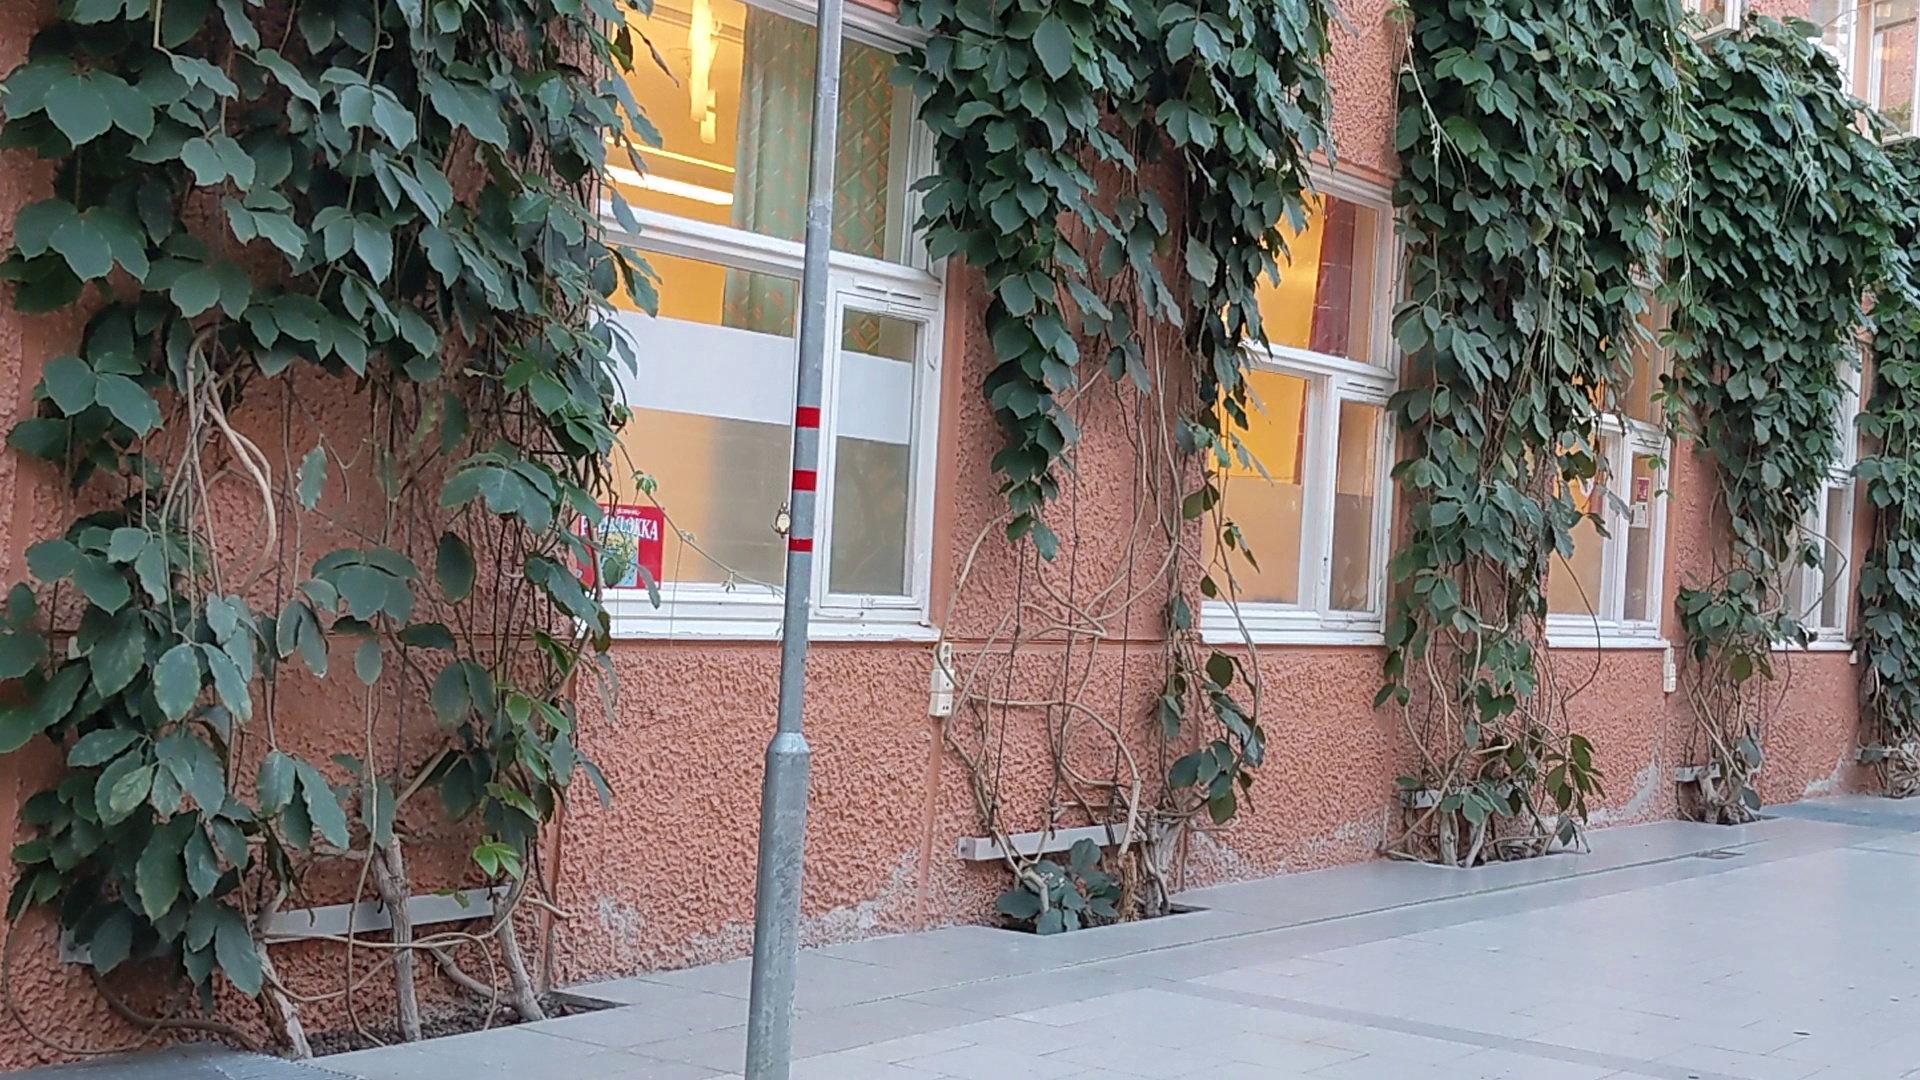
\includegraphics[width=0.7\textwidth]{img/video_frame_150/BG_Complex_150.jpg}
    \caption{Frame 150 from the complex wall background video}
    \label{fig:background_complex_wall}
\end{figure}

\subsubsection{Background with windows}
Also a similar shot to the complex wall, sharing a lot of the same characteristics, but with a bright shining window opening to the right back. This gives the algorithm a challenge with the different types of exposures in the image. This video also contains some movements from the people in the shot, which leads to this being the most dynamic shot. 

\begin{figure}[H]
    \centering
    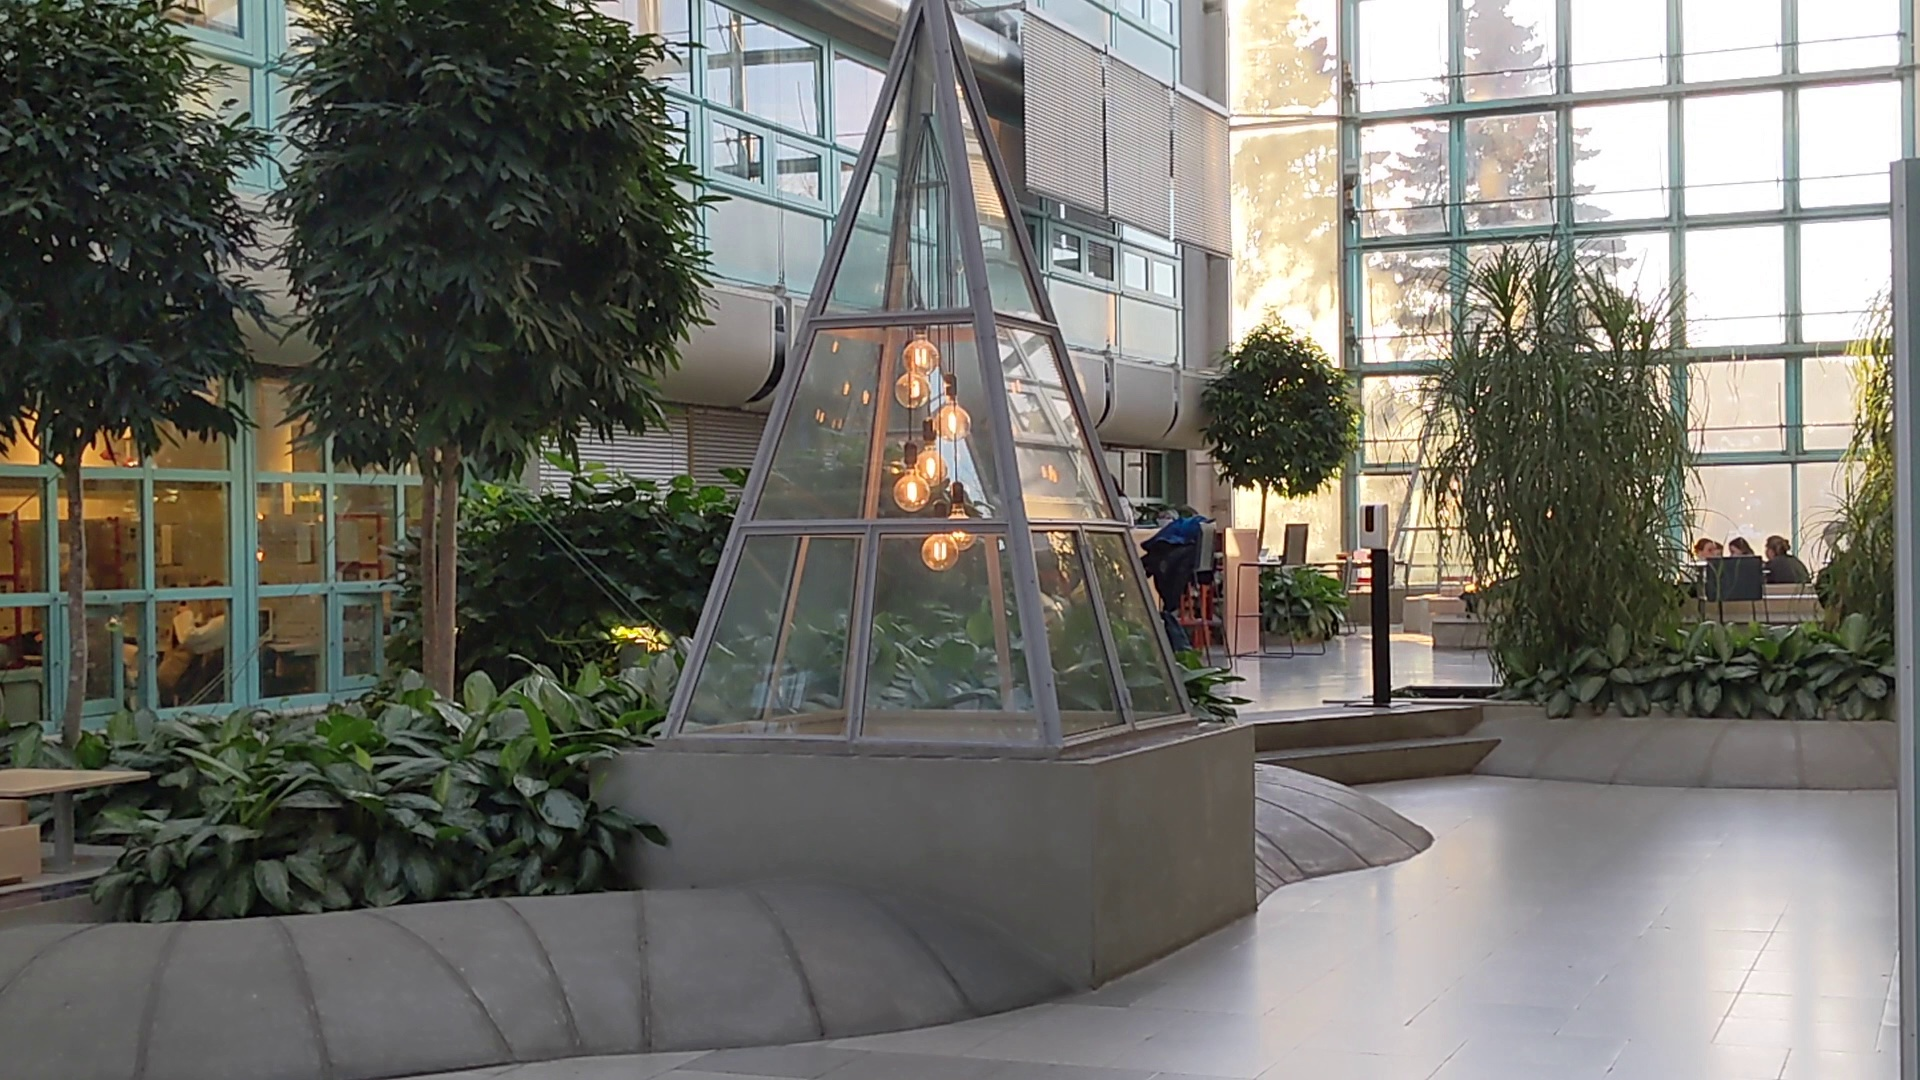
\includegraphics[width=0.7\textwidth]{img/video_frame_150/BG_Window_150.jpg}
    \caption{Frame 150 from the window wall background video}
    \label{fig:background_window_wall}
\end{figure}

\subsection{Foregrounds}\label{sec:foregrounds}
The foreground videos were constructed inside the Sense-IT laboratory at NTNU. \autoref{fig:placement} illustrates the setup and how the gear, described in \autoref{sec:hardware}, was placed. 

The placement of the ring lights were decided by trial and error to try to minimise the shadow casting from the actor onto the green screen. This step was important for easier chroma key post processing.

\begin{figure}[H]
  \centering
  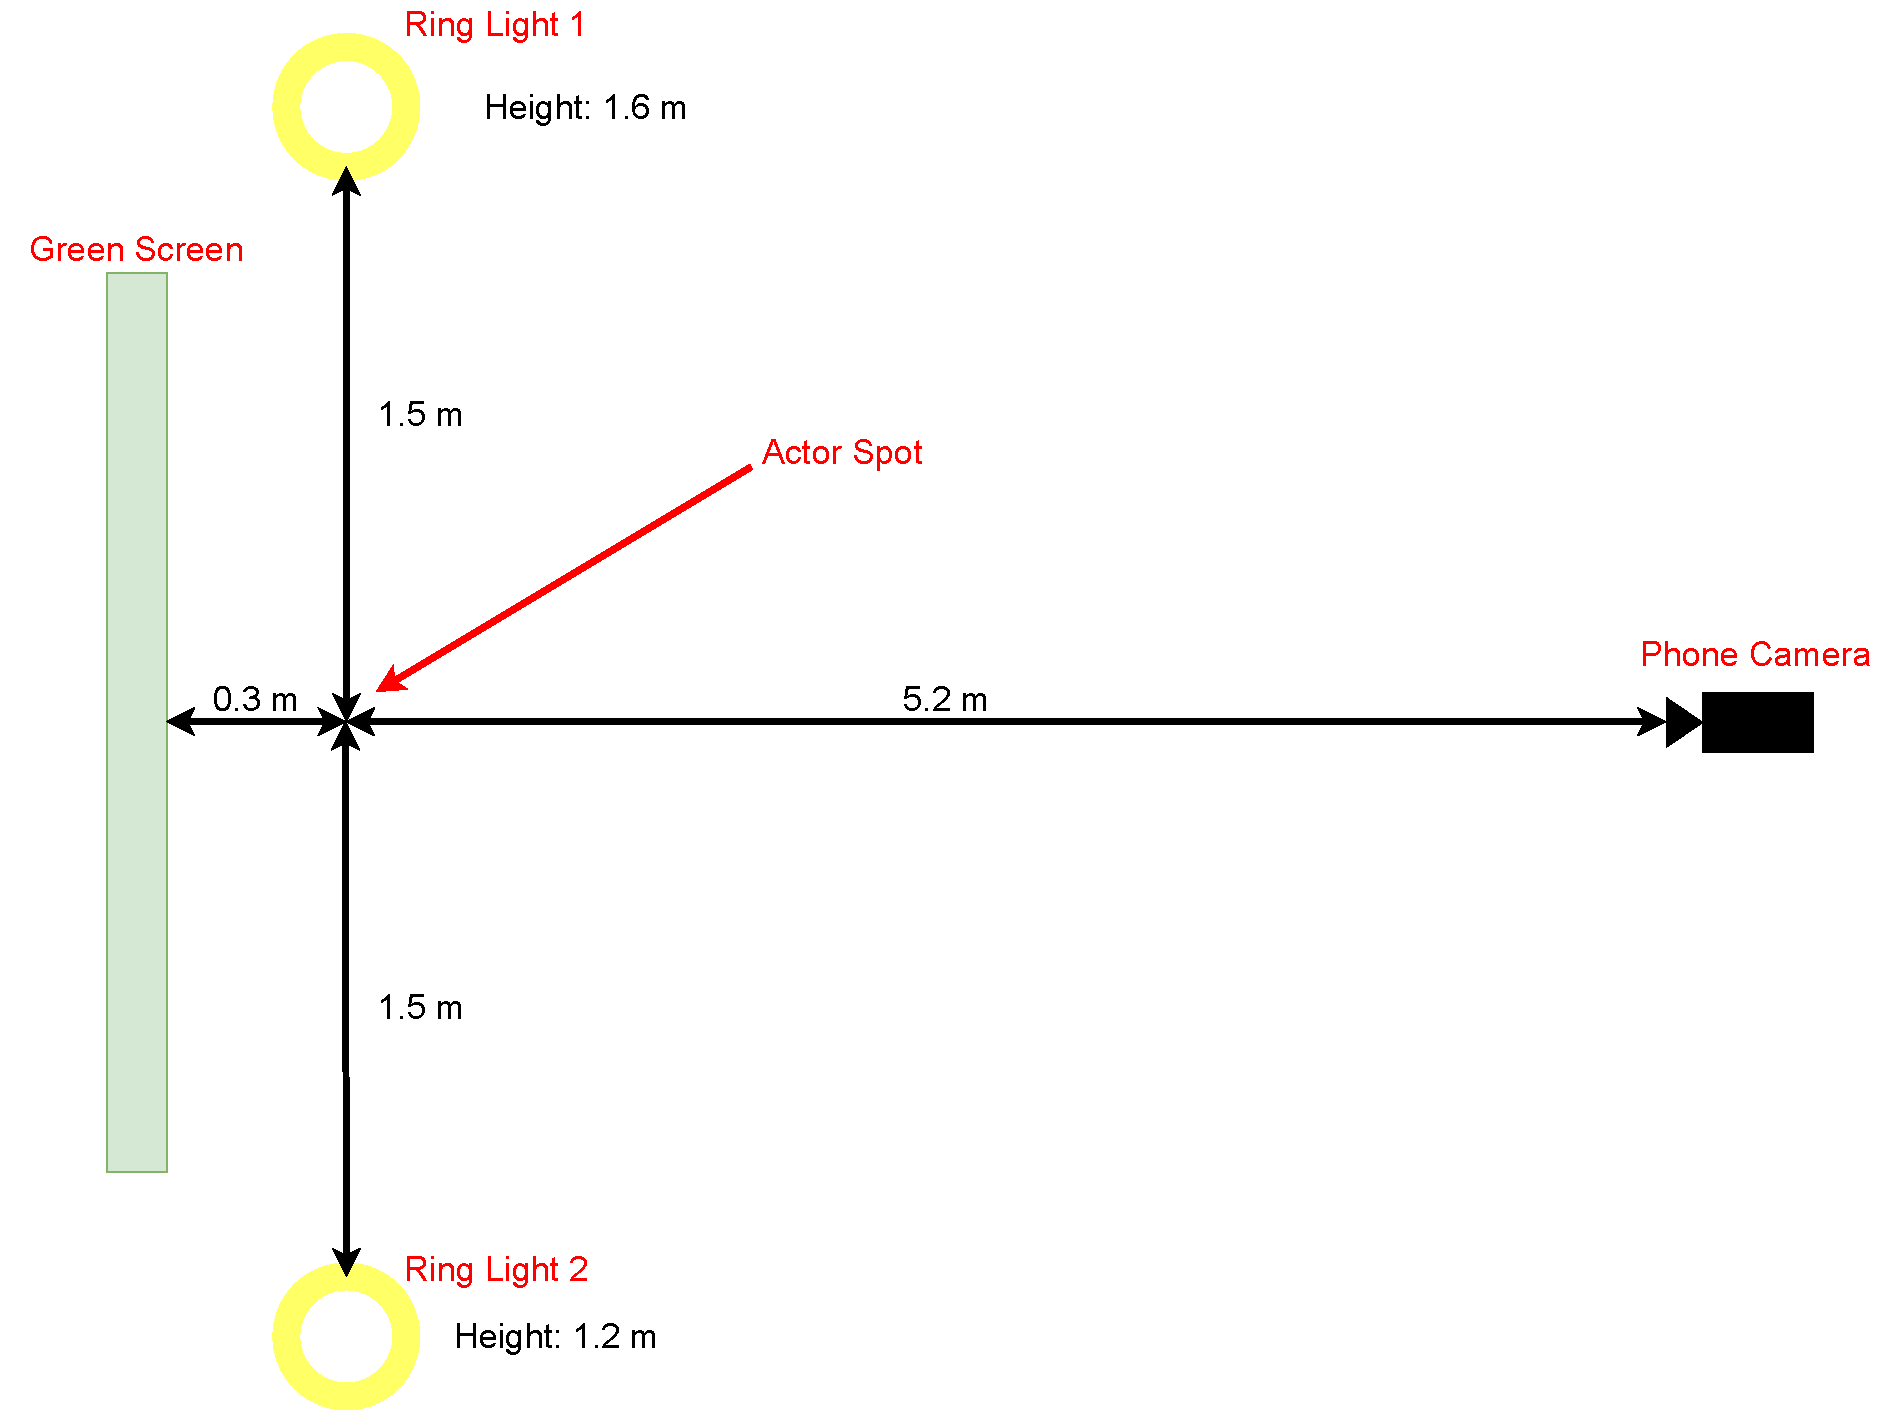
\includegraphics[width=\textwidth]{img/video_setup/placement.pdf}
  \caption{Placement of gear in the Sense-IT laboratory for the foreground shots}
  \label{fig:placement}
\end{figure}

\subsubsection{Person counting ten fingers}
This foreground was constructed to evaluate how well the machine learning algorithm handles the spacing between the fingers and how well it manages to segment these small areas.

\begin{figure}[H]
    \centering
    
\includegraphics[width=0.6\textwidth]{img/video_frame_150/FG_Counting-Fingers_150.jpg}
    \caption{Frame 150 from the finger counting video}
    \label{fig:foreground_counting}
\end{figure}


\subsubsection{Person wearing a light clothing rocking back and forth}
See how well the algorithm performs on a person wearing light coloured clothing since some of the backgrounds will have lighter elements in them. How does this compare to the dark clothing?

\begin{figure}[H]
    \centering
    
\includegraphics[width=0.6\textwidth]{img/video_frame_150/FG_Rocking-Light_150.jpg}
    \caption{Frame 150 from the light clothing video}
    \label{fig:foreground_light_clothing}
\end{figure}


\subsubsection{Person wearing a dark clothing rocking back and forth}
See how well the algorithm performs on a person wearing dark coloured clothing, since some of the backgrounds will have darker elements in them. How does this compare to the light clothing?

\begin{figure}[H]
    \centering
    
\includegraphics[width=0.6\textwidth]{img/video_frame_150/FG_Rocking-Dark_150.jpg}
    \caption{Frame 150 from the dark clothing video}
    \label{fig:foreground_dark_clothing}
\end{figure}


\subsubsection{Person displaying an object in their hands}
As we know from \autoref{sec:mlbfe}, the model is only trained on persons, but what happens if a person is holding an object, like a book? It is quite possible the \acrshort{mlbfe} is going to handle foreign objects in production. What will the \acrshort{mlbfe} do? Cut it out properly? Leave the object untouched?

\begin{figure}[H]
    \centering
    
\includegraphics[width=0.6\textwidth]{img/video_frame_150/FG_Showing-Object_150.jpg}
    \caption{Frame 150 from the showing object video}
    \label{fig:foreground_showing_object}
\end{figure}

\subsection{Final Video List}
After the combinations of the different foregrounds and backgrounds, we get the final video list from \autoref{tab:video_list}.

\begin{table}[H]
    \centering
    \begin{tabular}{|c|p{4cm}|p{4cm}|} 
         \hline
         \textbf{Video} & \textbf{Foreground} & \textbf{Background} \\ [0.5ex] 
         \hline\hline
         1 & Showing Object & Complex \\
         \hline
         2 & Showing Object & Window \\
         \hline
         3 & Showing Object & White Wall \\
         \hline
         4 & Rocking Dark & Complex \\
         \hline
         5 & Rocking Dark & Window \\
         \hline
         6 & Rocking Dark & White Wall \\
         \hline
         7 & Rocking Light & Complex \\
         \hline
         8 & Rocking Light & Window \\
         \hline
         9 & Rocking Light & White Wall \\
         \hline
         10 & Counting Fingers & Complex \\
         \hline
         11 & Counting Fingers & Window \\
         \hline
         12 & Counting Fingers & White Wall \\
         \hline
    \end{tabular}
    \caption{}
    \label{tab:video_list}
\end{table}


\section{Measures}
\subsection{Objective measures}
The resulting videos from figure \ref{fig:videos}b (chroma key video) and \ref{fig:videos}d (machine learning video) will be statistically compared and reviewed head to head. The chroma key video will be our truth table, while the frame from the machine learning video will be our input. 

To make the computations easier, we will convert our frames to binary images in black and white, where the background is black and the silhouette extraction is white. We will be using Python to retrieve the objective measures discussed in \autoref{sec:objective_measurement} for each frame. Additionally, the mean of each objective measure will be calculated for each video for an general evaluation of the video in its entirety. The developed code can be found in \autoref{cha:appendix-github}.



\subsection{Subjective measures}\label{sec:system_subjective}
A group of participants will be given a questionnaire to collect the subjective measures of the quality of the resulting videos from the \acrshort{mlbfe} processed videos presented in \autoref{fig:videos}d. The questionnaire will map the demographic to map the age, gender, education and occupation, to see the coverage of low level human influencing factors and to see our representation of people. Afterwards, they will be asked some questions for each video. The questions, with answers, are listed in \autoref{tab:q1}, \autoref{tab:q2} and \autoref{tab:q1}.

\begin{table}[H]
    \centering
    \begin{tabular}{ |c|c| } 
         \hline
             \textbf{Question 1} & How satisfied are you with the quality of the silhouette extraction? \\
         \hline
             \textbf{Answer} & \begin{tabular}{c} Completely satisfied \\ Very satisfied \\ Moderately satisfied \\ Slightly satisfied \\ Not at all satisfied \end{tabular} \\
         \hline
    \end{tabular}
    \caption{Question and answers for question 1}
    \label{tab:q1}
\end{table}


\begin{table}[H]
    \centering
    \begin{tabular}{ |c|c| } 
         \hline
             \textbf{Question 2} & Did you notice any artefacts with the silhouette extraction? \\
         \hline
             \textbf{Answer} & \begin{tabular}{c} Extremely noticeable \\ Very noticeable \\ Moderately noticeable \\ Slightly noticeable \\ Not at all noticeable \end{tabular} \\
         \hline
    \end{tabular}
    \caption{Question and answers for question 2}
    \label{tab:q2}
\end{table}

\begin{table}[H]
    \centering
    \begin{tabular}{ |c|c| } 
         \hline
             \textbf{Question 3} & Do you think the artefacts were annoying? \\
         \hline
             \textbf{Answer} & \begin{tabular}{c} Extremely annoying \\ Very annoying \\ Moderately annoying \\ Slightly annoying \\ Not at all annoying \end{tabular} \\
         \hline
    \end{tabular}
    \caption{Question and answers for question 3}
    \label{tab:q3}
\end{table}


The participants will be able to answer the questions with a fitting five point Likert scale and also be able to add additional qualitative feedback in the end if wanted. 

The rating will be done using Google Forms. An export of the questionnaire is presented in \autoref{cha:appendix-questionnaire}. The videos have been implemented into the questionnaire as an unlisted YouTube video uploaded to a newly created account for the survey purpose. This has been done to prevent any targeted recommendations and other recommendations provided by the YouTube algorithms. 

The order of the videos presented in the questionnaire was decided by a shuffling the order of the videos through a randomising function, with the final order presented in \autoref{tab:order}. This was done to prevent the participants to see the same foreground videos after one another. Using this setup, we will be able to test on a lot of participants, which hopefully will yield a more fair and even result. 

\begin{table}[H]
    \centering
    \begin{tabular}{ |c|c|c|c|c|c|c|c|c|c|c|c|c| } 
         \hline
             \textbf{Video name number} & 1 & 2 & 3 & 4 & 5 & 6 & 7 & 8 & 9 & 10 & 11 & 12 \\
         \hline
             \textbf{Shuffled video order} & 10 & 9 & 3 & 7 & 6 & 2 & 1 & 12 & 8 & 4 & 11 & 5 \\
         \hline
    \end{tabular}
    \caption{Order of the videos in the questionnaire}
    \label{tab:order}
\end{table}

\section{Hardware}\label{sec:hardware}
\begin{table}[H]
    \centering
    \begin{tabular}{|p{2cm}|p{1.5cm}|p{3.5cm}|p{3cm}|} 
         \hline
         \textbf{What} & \textbf{Model} & \textbf{Specifications} & \textbf{Comment} \\ [0.5ex] 
         \hline\hline
         Video Camera Mobile Phone & Google Pixel 5 & Resolution: 1920x1080 \newline Codec: H.264, AAC, avc1 \newline Color Profile: (5-1-6) \newline Rec.601 (PAL) & Phone used to replicate the normal use case for the AdMiRe project \\
         \hline
         Editing machine & MacBook Air & 1.1GHz 4-core i5, 16GB RAM & Editing software: Final Cut Pro 10.6 \\
         \hline
         Machine learning machine & N.A. & 3.6GHz 8-core i7-7700, RTX A6000 & Running Ubuntu \\
         \hline
         Green Screen & Elgato & Extended: 148x180 cm & Feet get cut off \\
         \hline
         Ring Lights & Elgato & 2900-7000K, 2500 lm, 45W & One for left and right side. To remove shadows from green screen \\
         \hline
         Tripods & Any & N.A. & One for each ring light, and one for camera \\ [1ex] 
         \hline
    \end{tabular}
    \caption{Hardware specifications}
    \label{tab:harware}
\end{table}

%!TEX root = ../Thesis.tex
\chapter{Results}\label{cha:results}
%
\textcolor{red}{The results chapter should simply present the results of applying the methods presented in the method chapter without further ado. This chapter will typically contain many graphs, tables, etc. Sometimes it is natural to discuss the results as they are presented, combining them into a `Results and Discussion' chapter, but more often they are kept separate.}

This chapter will be used to look at the results from the objective and subjective measures and compare these against each other. There were a total of 54 participants which answered the subjective questionnaire. \autoref{fig:age} shows the age distribution of the participants, while \autoref{fig:gender} shows the gender distribution. \autoref{fig:occupation} and \autoref{fig:education} shows what type of occupation and education the participants had. 

For the statistical measures we plotted each of the questions to each video in histograms, along with error bars giving the standard deviation of the data set. The standard deviation was used to check the spread and variability of the data. We further looked at the histogram data manually to gather information from the result, as well as presenting the mean score, percentage of full score and the standard deviation in a table for easier evaluation and comparison against the objective measures.

\begin{figure}
\centering
\begin{minipage}{.5\textwidth}
  \centering
  \includegraphics[width=\linewidth]{img/subjective_measures/demographic/age_plot .pdf}
  \captionof{figure}{Age Distribution}
  \label{fig:age}
\end{minipage}%
\begin{minipage}{.5\textwidth}
  \centering
  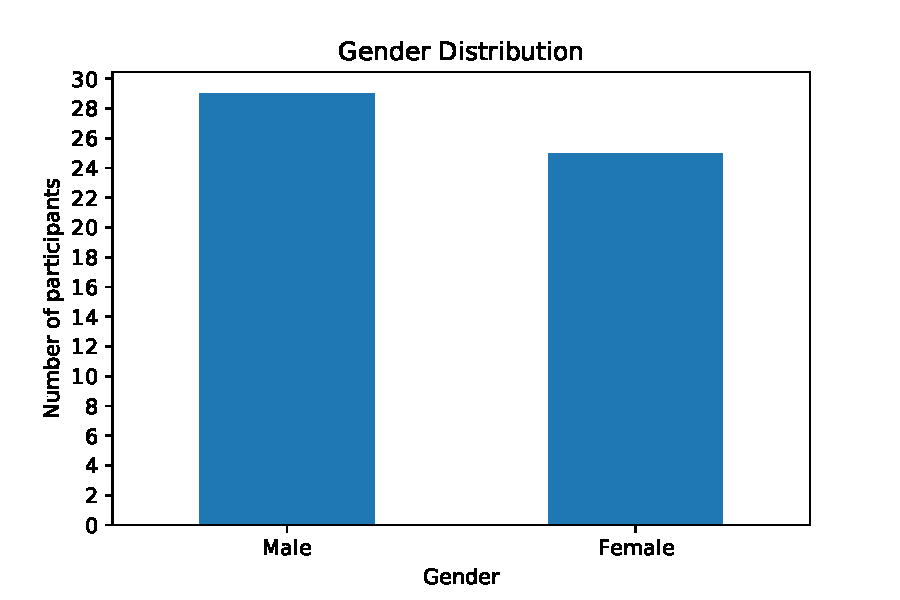
\includegraphics[width=\linewidth]{img/subjective_measures/demographic/gender_plot.pdf}
  \captionof{figure}{Gender Distribution}
  \label{fig:gender}
\end{minipage}
\end{figure}


\begin{figure}
\centering
\begin{minipage}{.5\textwidth}
  \centering
  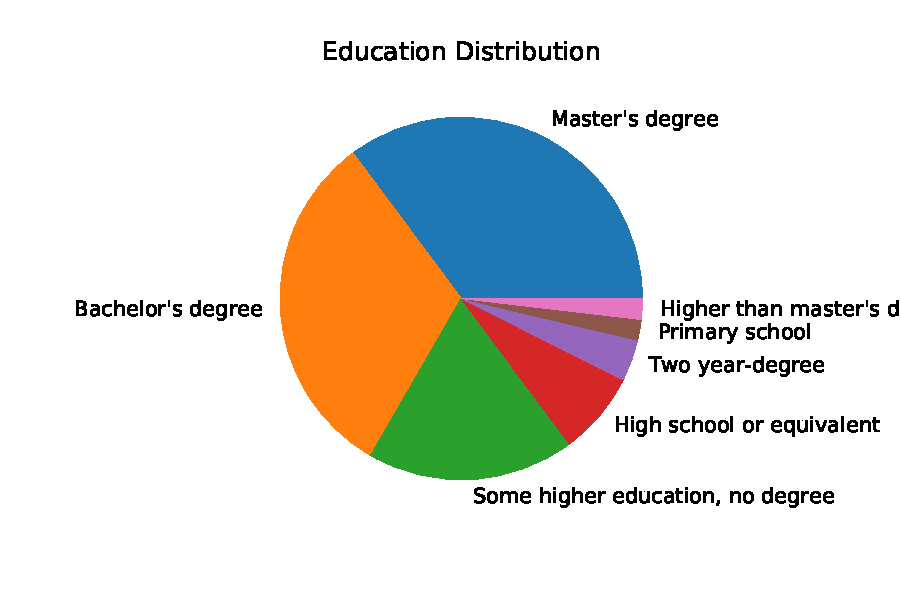
\includegraphics[width=\linewidth]{img/subjective_measures/demographic/education.pdf}
  \captionof{figure}{Education Distribution}
  \label{fig:education}
\end{minipage}%
\begin{minipage}{.5\textwidth}
  \centering
  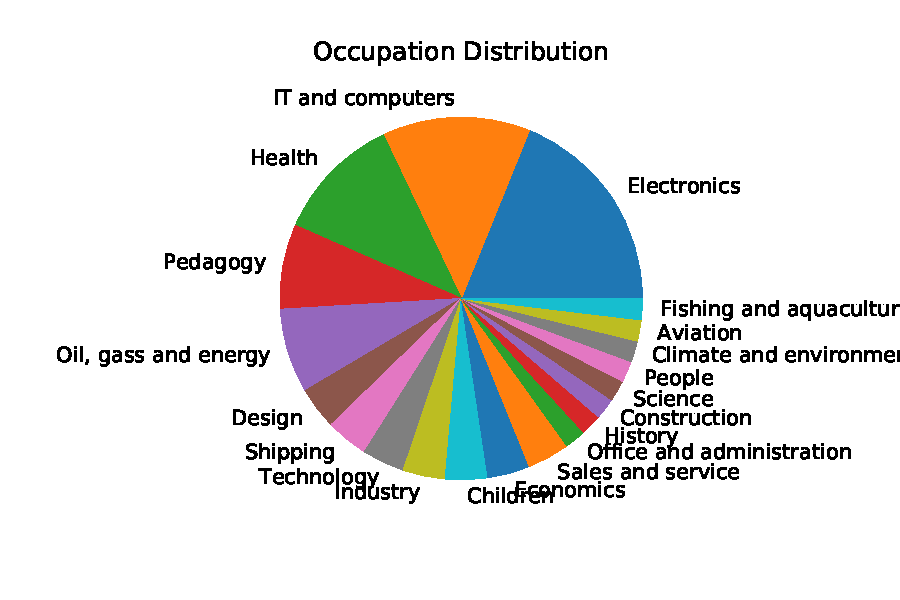
\includegraphics[width=\linewidth]{img/subjective_measures/demographic/occupations.pdf}
  \captionof{figure}{Occupation Distribution}
  \label{fig:occupation}
\end{minipage}
\end{figure}



\section{Video 1}
\subsection{Objective Measures}

\begin{minipage}[c]{0.475\textwidth}
\begin{table}[H]
    \centering
    \begin{tabular}{||c c c||} 
        \hline
        \acrshort{iou} & \acrshort{dc} & \acrshort{pa} \\ [0.5ex] 
        \hline\hline
        93.590\% & 96.668\% & 99.220\% \\ [1ex] 
        \hline
    \end{tabular}
    \caption{Average metrics}
    \label{tab:metrics_video_1}
\end{table}
\end{minipage}
\begin{minipage}[c]{0.475\textwidth}
\begin{table}[H]
    \centering
    \begin{tabular}{||c c c||} 
        \hline
        \acrshort{tp} & \acrshort{tn} & \acrshort{fpn} \\ [0.5ex] 
        \hline\hline
        232890 & 1824538 & 16170 \\ [1ex] 
        \hline
    \end{tabular}
    \caption{Average pixel classification}
    \label{tab:pixels_video_1}
\end{table}
\end{minipage}

\subsection{Subjective Measures}

\begin{figure}[H]
    \centering
    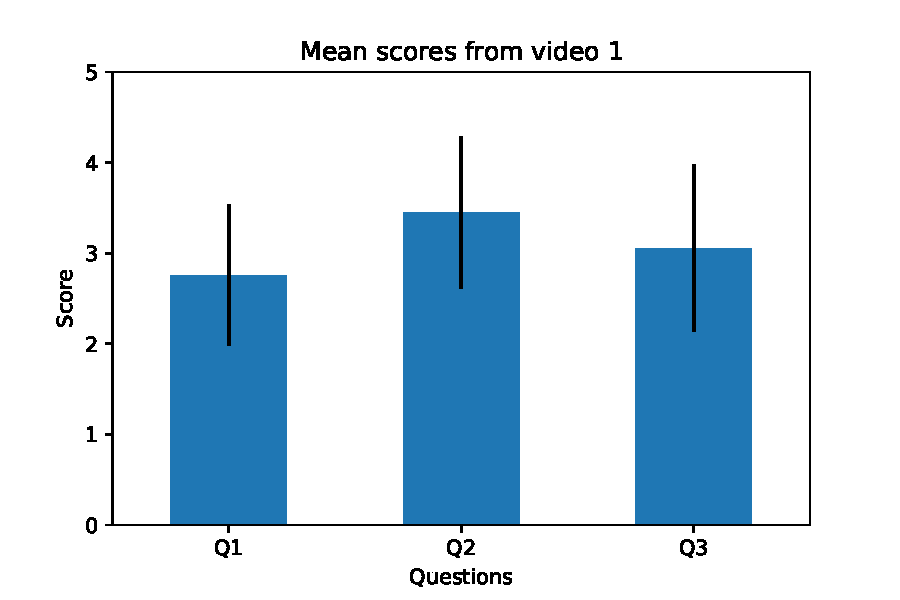
\includegraphics[width=0.6\textwidth]{img/subjective_measures/analysis/video_1.pdf}
    \caption{Subjective rating on video 1}
    \label{fig:visual_subj_vid1}
\end{figure}

\begin{table}[H]
    \centering
    \begin{tabular}{|c|c c c|} 
        \hline
           & \textbf{Mean Score} & \textbf{Percentage of full score} & \textbf{Standard Deviation} \\ [0.5ex] 
        \hline
        Q1 & 2.759 & 55.185\% & 0.775 \\ [1ex] 
        Q2 & 3.444 & 68.889\% & 0.839 \\ [1ex] 
        Q3 & 3.056 & 61.111\% & 0.920 \\ [1ex] 
        \hline
    \end{tabular}
    \caption{Numerical metrics from subjective rating in video 1}
    \label{tab:numerical_subj_vid1}
\end{table}

%------------------------------------

%------------------------------------

\section{Video 2}
\subsection{Objective Measures}

\begin{minipage}[c]{0.475\textwidth}
\begin{table}[H]
    \centering
    \begin{tabular}{||c c c||} 
        \hline
        \acrshort{iou} & \acrshort{dc} & \acrshort{pa} \\ [0.5ex] 
        \hline\hline
        94.097\% & 96.944\% & 99.281\% \\ [1ex] 
        \hline
    \end{tabular}
    \caption{Average metrics}
    \label{tab:metrics_video_2}
\end{table}
\end{minipage}
\begin{minipage}[c]{0.475\textwidth}
\begin{table}[H]
    \centering
    \begin{tabular}{||c c c||} 
        \hline
        \acrshort{tp} & \acrshort{tn} & \acrshort{fpn} \\ [0.5ex] 
        \hline\hline
        234287 & 1824412 & 14901 \\ [1ex] 
        \hline
    \end{tabular}
    \caption{Average pixel classification}
    \label{tab:pixels_video_11}
\end{table}
\end{minipage}

\subsection{Subjective Measures}

\begin{figure}[H]
    \centering
    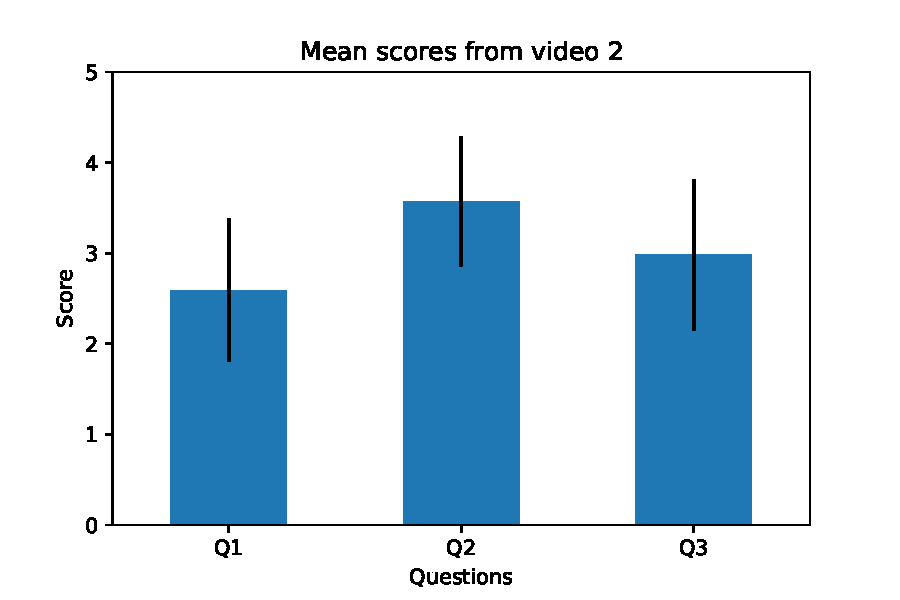
\includegraphics[width=0.6\textwidth]{img/subjective_measures/analysis/video_2.pdf}
    \caption{Subjective rating on video 2}
    \label{fig:visual_subj_vid2}
\end{figure}

\begin{table}[H]
    \centering
    \begin{tabular}{|c|c c c|} 
        \hline
           & \textbf{Mean Score} & \textbf{Percentage of full score} & \textbf{Standard Deviation} \\ [0.5ex] 
        \hline
        Q1 & 2.593 & 51.852\% & 0.790 \\ [1ex] 
        Q2 & 3.574 & 71.481\% & 0.716 \\ [1ex] 
        Q3 & 2.981 & 59.630\% & 0.835 \\ [1ex] 
        \hline
    \end{tabular}
    \caption{Numerical metrics from subjective rating in video 2}
    \label{tab:numerical_subj_vid2}
\end{table}

%------------------------------------

%------------------------------------

\section{Video 3}
\subsection{Objective Measures}

\begin{minipage}[c]{0.475\textwidth}
\begin{table}[H]
    \centering
    \begin{tabular}{||c c c||} 
        \hline
        \acrshort{iou} & \acrshort{dc} & \acrshort{pa} \\ [0.5ex] 
        \hline\hline
        95.096\% & 97.486\% & 99.406\% \\ [1ex] 
        \hline
    \end{tabular}
    \caption{Average metrics}
    \label{tab:metrics_video_3}
\end{table}
\end{minipage}
\begin{minipage}[c]{0.475\textwidth}
\begin{table}[H]
    \centering
    \begin{tabular}{||c c c||} 
        \hline
        \acrshort{tp} & \acrshort{tn} & \acrshort{fpn} \\ [0.5ex] 
        \hline\hline
        237919 & 1823370 & 12310 \\ [1ex] 
        \hline
    \end{tabular}
    \caption{Average pixel classification}
    \label{tab:pixels_video_3}
\end{table}
\end{minipage}

\subsection{Subjective Measures}

\begin{figure}[H]
    \centering
    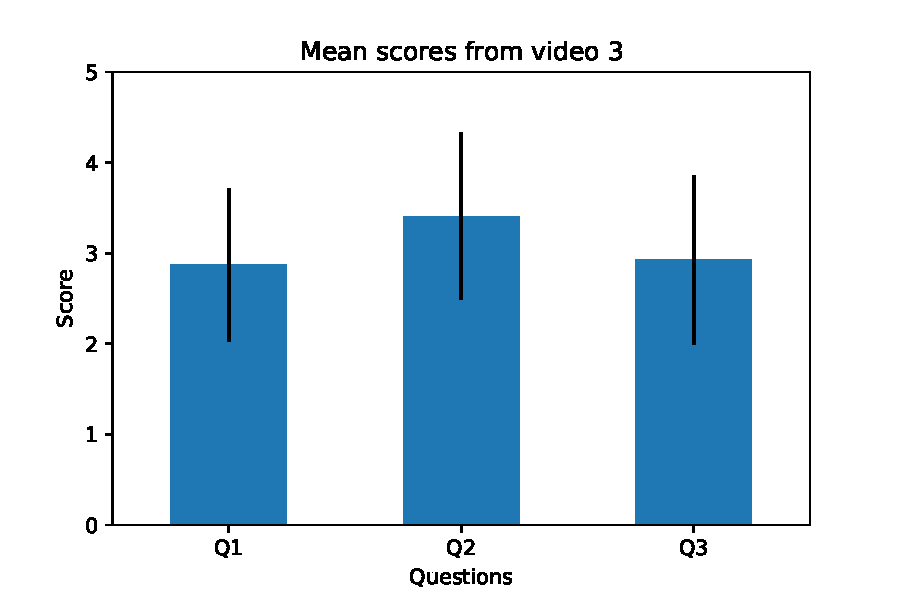
\includegraphics[width=0.6\textwidth]{img/subjective_measures/analysis/video_3.pdf}
    \caption{Subjective rating on video 3}
    \label{fig:visual_subj_vid3}
\end{figure}

\begin{table}[H]
    \centering
    \begin{tabular}{|c|c c c|} 
        \hline
           & \textbf{Mean Score} & \textbf{Percentage of full score} & \textbf{Standard Deviation} \\ [0.5ex] 
        \hline
        Q1 & 2.870 & 57.407\% & 0.848 \\ [1ex] 
        Q2 & 3.407 & 68.148\% & 0.922 \\ [1ex] 
        Q3 & 2.926 & 58.519\% & 0.929 \\ [1ex] 
        \hline
    \end{tabular}
    \caption{Numerical metrics from subjective rating in video 3}
    \label{tab:numerical_subj_vid3}
\end{table}



%------------------------------------

%------------------------------------

\section{Video 4}
\subsection{Objective Measures}

\begin{minipage}[c]{0.475\textwidth}
\begin{table}[H]
    \centering
    \begin{tabular}{||c c c||} 
        \hline
        \acrshort{iou} & \acrshort{dc} & \acrshort{pa} \\ [0.5ex] 
        \hline\hline
        94.719\% & 97.287\% & 99.354\% \\ [1ex] 
        \hline
    \end{tabular}
    \caption{Average metrics}
    \label{tab:metrics_video_4}
\end{table}
\end{minipage}
\begin{minipage}[c]{0.475\textwidth}
\begin{table}[H]
    \centering
    \begin{tabular}{||c c c||} 
        \hline
        \acrshort{tp} & \acrshort{tn} & \acrshort{fpn} \\ [0.5ex] 
        \hline\hline
        240444 & 1819753 & 13403 \\ [1ex] 
        \hline
    \end{tabular}
    \caption{Average pixel classification}
    \label{tab:pixels_video_4}
\end{table}
\end{minipage}

\subsection{Subjective Measures}

\begin{figure}[H]
    \centering
    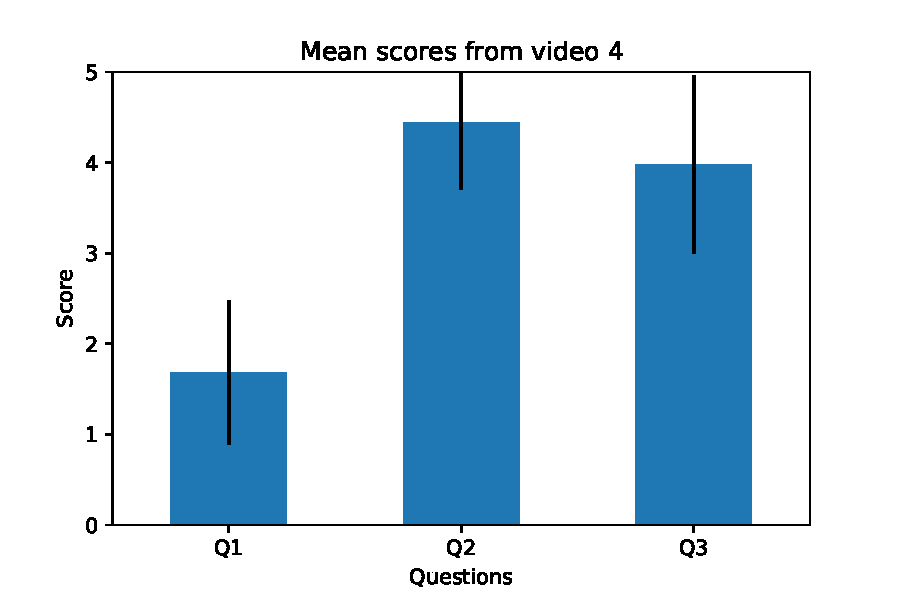
\includegraphics[width=0.6\textwidth]{img/subjective_measures/analysis/video_4.pdf}
    \caption{Subjective rating on video 4}
    \label{fig:visual_subj_vid4}
\end{figure}

\begin{table}[H]
    \centering
    \begin{tabular}{|c|c c c|} 
        \hline
           & \textbf{Mean Score} & \textbf{Percentage of full score} & \textbf{Standard Deviation} \\ [0.5ex] 
        \hline
        Q1 & 1.685 & 33.704\% & 0.797 \\ [1ex] 
        Q2 & 4.444 & 88.889\% & 0.744 \\ [1ex] 
        Q3 & 3.981 & 79.630\% & 0.981 \\ [1ex] 
        \hline
    \end{tabular}
    \caption{Numerical metrics from subjective rating in video 4}
    \label{tab:numerical_subj_vid4}
\end{table}


%------------------------------------

%------------------------------------

\section{Video 5}
\subsection{Objective Measures}

\begin{minipage}[c]{0.475\textwidth}
\begin{table}[H]
    \centering
    \begin{tabular}{||c c c||} 
        \hline
        \acrshort{iou} & \acrshort{dc} & \acrshort{pa} \\ [0.5ex] 
        \hline\hline
        94.812\% & 97.336\% & 99.366\% \\ [1ex] 
        \hline
    \end{tabular}
    \caption{Average metrics}
    \label{tab:metrics_video_5}
\end{table}
\end{minipage}
\begin{minipage}[c]{0.475\textwidth}
\begin{table}[H]
    \centering
    \begin{tabular}{||c c c||} 
        \hline
        \acrshort{tp} & \acrshort{tn} & \acrshort{fpn} \\ [0.5ex] 
        \hline\hline
        240427 & 1820023 & 13150 \\ [1ex] 
        \hline
    \end{tabular}
    \caption{Average pixel classification}
    \label{tab:pixels_video_5}
\end{table}
\end{minipage}

\subsection{Subjective Measures}

\begin{figure}[H]
    \centering
    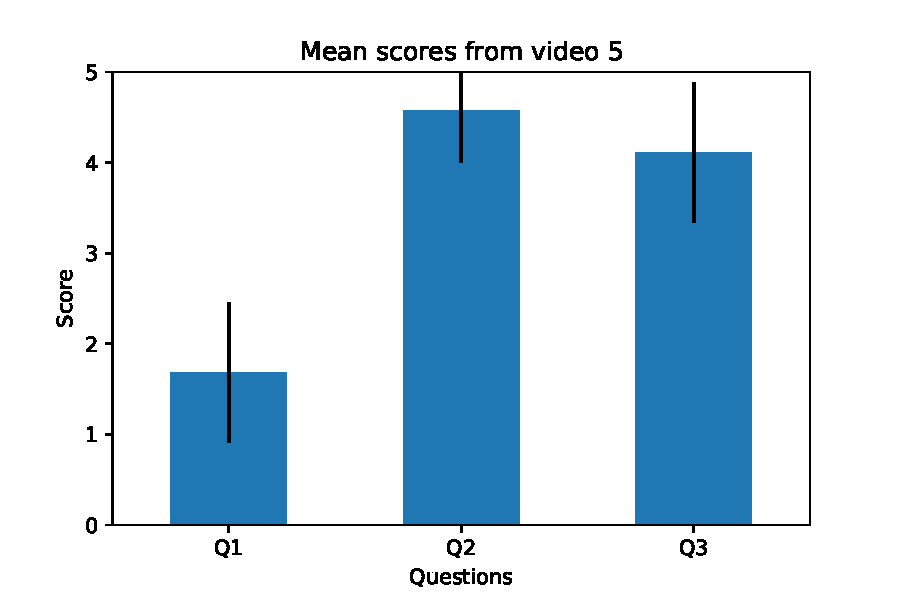
\includegraphics[width=0.6\textwidth]{img/subjective_measures/analysis/video_5.pdf}
    \caption{Subjective rating on video 5}
    \label{fig:visual_subj_vid5}
\end{figure}

\begin{table}[H]
    \centering
    \begin{tabular}{|c|c c c|} 
        \hline
           & \textbf{Mean Score} & \textbf{Percentage of full score} & \textbf{Standard Deviation} \\ [0.5ex] 
        \hline
        Q1 & 1.685 & 33.704\% & 0.773 \\ [1ex] 
        Q2 & 4.574 & 91.481\% & 0.570 \\ [1ex] 
        Q3 & 4.113 & 82.264\% & 0.776 \\ [1ex] 
        \hline
    \end{tabular}
    \caption{Numerical metrics from subjective rating in video 5}
    \label{tab:numerical_subj_vid5}
\end{table}


%------------------------------------

%------------------------------------
\section{Video 6}
\subsection{Objective Measures}

\begin{minipage}[c]{0.475\textwidth}
\begin{table}[H]
    \centering
    \begin{tabular}{||c c c||} 
        \hline
        \acrshort{iou} & \acrshort{dc} & \acrshort{pa} \\ [0.5ex] 
        \hline\hline
        94.239\% & 97.033\% & 99.292\% \\ [1ex] 
        \hline
    \end{tabular}
    \caption{Average metrics}
    \label{tab:metrics_video_6}
\end{table}
\end{minipage}
\begin{minipage}[c]{0.475\textwidth}
\begin{table}[H]
    \centering
    \begin{tabular}{||c c c||} 
        \hline
        \acrshort{tp} & \acrshort{tn} & \acrshort{fpn} \\ [0.5ex] 
        \hline\hline
        240430 & 1818482 & 14687 \\ [1ex] 
        \hline
    \end{tabular}
    \caption{Average pixel classification}
    \label{tab:pixels_video_6}
\end{table}
\end{minipage}

\subsection{Subjective Measures}

\begin{figure}[H]
    \centering
    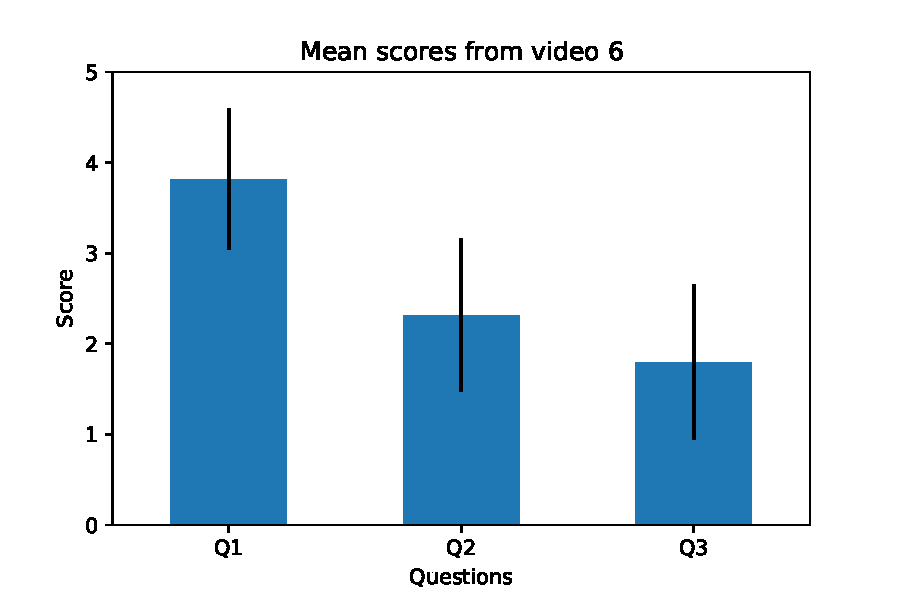
\includegraphics[width=0.6\textwidth]{img/subjective_measures/analysis/video_6.pdf}
    \caption{Subjective rating on video 6}
    \label{fig:visual_subj_vid6}
\end{figure}

\begin{table}[H]
    \centering
    \begin{tabular}{|c|c c c|} 
        \hline
           & \textbf{Mean Score} & \textbf{Percentage of full score} & \textbf{Standard Deviation} \\ [0.5ex] 
        \hline
        Q1 & 3.815 & 76.296\% & 0.779 \\ [1ex] 
        Q2 & 2.315 & 46.296\% & 0.843 \\ [1ex] 
        Q3 & 1.796 & 35.926\% & 0.855 \\ [1ex] 
        \hline
    \end{tabular}
    \caption{Numerical metrics from subjective rating in video 6}
    \label{tab:numerical_subj_vid6}
\end{table}

%------------------------------------

%------------------------------------

\section{Video 7}
\subsection{Objective Measures}

\begin{minipage}[c]{0.475\textwidth}
\begin{table}[H]
    \centering
    \begin{tabular}{||c c c||} 
        \hline
        \acrshort{iou} & \acrshort{dc} & \acrshort{pa} \\ [0.5ex] 
        \hline\hline
        93.909\% & 96.855\% & 99.216\% \\ [1ex] 
        \hline
    \end{tabular}
    \caption{Average metrics}
    \label{tab:metrics_video_7}
\end{table}
\end{minipage}
\begin{minipage}[c]{0.475\textwidth}
\begin{table}[H]
    \centering
    \begin{tabular}{||c c c||} 
        \hline
        \acrshort{tp} & \acrshort{tn} & \acrshort{fpn} \\ [0.5ex] 
        \hline\hline
        249856 & 1807490 & 16253 \\ [1ex] 
        \hline
    \end{tabular}
    \caption{Average pixel classification}
    \label{tab:pixels_video_7}
\end{table}
\end{minipage}

\subsection{Subjective Measures}

\begin{figure}[H]
    \centering
    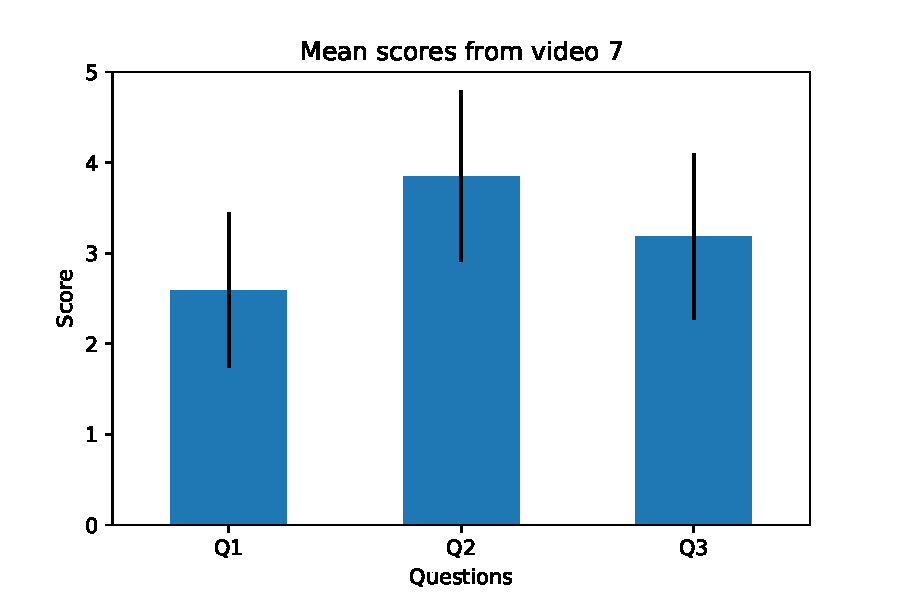
\includegraphics[width=0.6\textwidth]{img/subjective_measures/analysis/video_7.pdf}
    \caption{Subjective rating on video 7}
    \label{fig:visual_subj_vid7}
\end{figure}

\begin{table}[H]
    \centering
    \begin{tabular}{|c|c c c|} 
        \hline
           & \textbf{Mean Score} & \textbf{Percentage of full score} & \textbf{Standard Deviation} \\ [0.5ex] 
        \hline
        Q1 & 2.593 & 51.852\% & 0.858 \\ [1ex] 
        Q2 & 3.852 & 77.037\% & 0.940 \\ [1ex] 
        Q3 & 3.185 & 63.704\% & 0.913 \\ [1ex] 
        \hline
    \end{tabular}
    \caption{Numerical metrics from subjective rating in video 7}
    \label{tab:numerical_subj_vid7}
\end{table}

%------------------------------------

%------------------------------------

\section{Video 8}
\subsection{Objective Measures}

\begin{minipage}[c]{0.475\textwidth}
\begin{table}[H]
    \centering
    \begin{tabular}{||c c c||} 
        \hline
        \acrshort{iou} & \acrshort{dc} & \acrshort{pa} \\ [0.5ex] 
        \hline\hline
        94.749\% & 97.303\% & 99.332\% \\ [1ex] 
        \hline
    \end{tabular}
    \caption{Average metrics}
    \label{tab:metrics_video_8}
\end{table}
\end{minipage}
\begin{minipage}[c]{0.475\textwidth}
\begin{table}[H]
    \centering
    \begin{tabular}{||c c c||} 
        \hline
        \acrshort{tp} & \acrshort{tn} & \acrshort{fpn} \\ [0.5ex] 
        \hline\hline
        249735 & 1810021 & 13844 \\ [1ex] 
        \hline
    \end{tabular}
    \caption{Average pixel classification}
    \label{tab:pixels_video_8}
\end{table}
\end{minipage}

\subsection{Subjective Measures}

\begin{figure}[H]
    \centering
    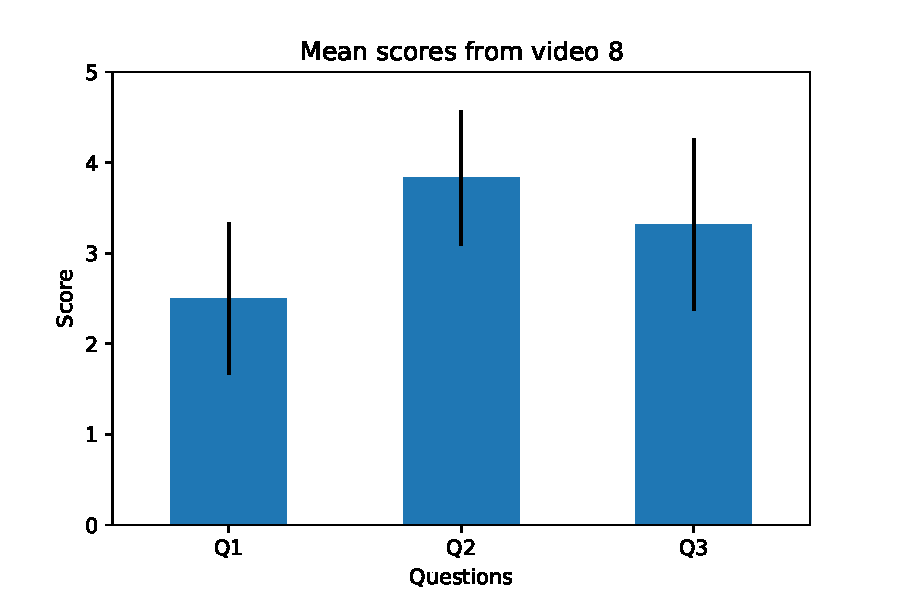
\includegraphics[width=0.6\textwidth]{img/subjective_measures/analysis/video_8.pdf}
    \caption{Subjective rating on video 8}
    \label{fig:visual_subj_vid8}
\end{figure}

\begin{table}[H]
    \centering
    \begin{tabular}{|c|c c c|} 
        \hline
           & \textbf{Mean Score} & \textbf{Percentage of full score} & \textbf{Standard Deviation} \\ [0.5ex] 
        \hline
        Q1 & 2.500 & 50.000\% & 0.841 \\ [1ex] 
        Q2 & 3.833 & 76.667\% & 0.746 \\ [1ex] 
        Q3 & 3.315 & 66.296\% & 0.948 \\ [1ex] 
        \hline
    \end{tabular}
    \caption{Numerical metrics from subjective rating in video 8}
    \label{tab:numerical_subj_vid8}
\end{table}

%------------------------------------

%------------------------------------

\section{Video 9}
\subsection{Objective Measures}

\begin{minipage}[c]{0.475\textwidth}
\begin{table}[H]
    \centering
    \begin{tabular}{||c c c||} 
        \hline
        \acrshort{iou} & \acrshort{dc} & \acrshort{pa} \\ [0.5ex] 
        \hline\hline
        93.687\% & 96.740\% & 99.187\% \\ [1ex] 
        \hline
    \end{tabular}
    \caption{Average metrics}
    \label{tab:metrics_video_9}
\end{table}
\end{minipage}
\begin{minipage}[c]{0.475\textwidth}
\begin{table}[H]
    \centering
    \begin{tabular}{||c c c||} 
        \hline
        \acrshort{tp} & \acrshort{tn} & \acrshort{fpn} \\ [0.5ex] 
        \hline\hline
        250392 & 1806340 & 16867 \\ [1ex] 
        \hline
    \end{tabular}
    \caption{Average pixel classification}
    \label{tab:pixels_video_9}
\end{table}
\end{minipage}

\subsection{Subjective Measures}

\begin{figure}[H]
    \centering
    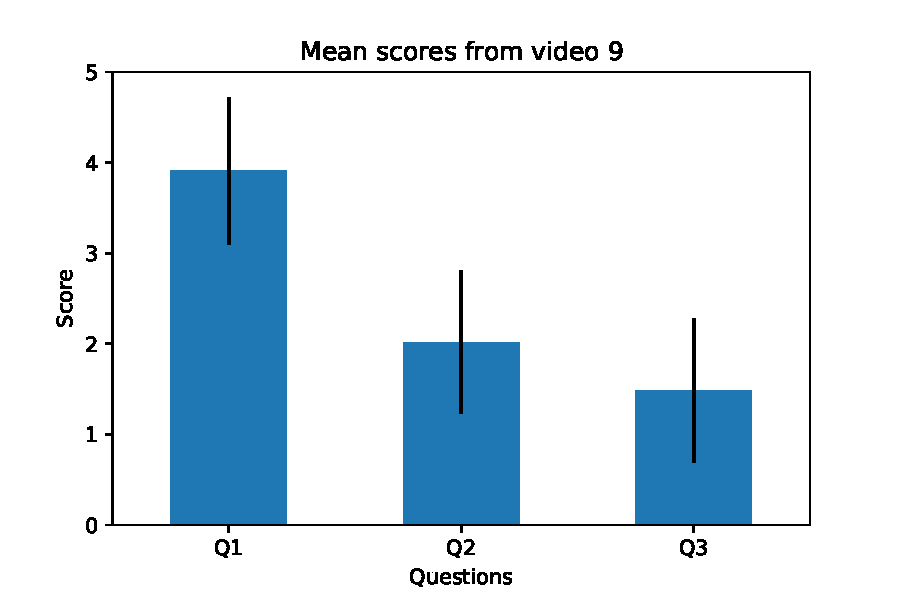
\includegraphics[width=0.6\textwidth]{img/subjective_measures/analysis/video_9.pdf}
    \caption{Subjective rating on video 9}
    \label{fig:visual_subj_vid9}
\end{figure}

\begin{table}[H]
    \centering
    \begin{tabular}{|c|c c c|} 
        \hline
           & \textbf{Mean Score} & \textbf{Percentage of full score} & \textbf{Standard Deviation} \\ [0.5ex] 
        \hline
        Q1 & 3.907 & 78.148\% & 0.807 \\ [1ex] 
        Q2 & 2.019 & 40.370\% & 0.789 \\ [1ex] 
        Q3 & 1.481 & 29.630\% & 0.795 \\ [1ex] 
        \hline
    \end{tabular}
    \caption{Numerical metrics from subjective rating in video 9}
    \label{tab:numerical_subj_vid9}
\end{table}

%------------------------------------

%------------------------------------


\section{Video 10}
\subsection{Objective Measures}

\begin{minipage}[c]{0.475\textwidth}
\begin{table}[H]
    \centering
    \begin{tabular}{||c c c||} 
        \hline
        \acrshort{iou} & \acrshort{dc} & \acrshort{pa} \\ [0.5ex] 
        \hline\hline
        93.982\% & 96.897\% & 99.240\% \\ [1ex] 
        \hline
    \end{tabular}
    \caption{Average metrics}
    \label{tab:metrics_video_10}
\end{table}
\end{minipage}
\begin{minipage}[c]{0.475\textwidth}
\begin{table}[H]
    \centering
    \begin{tabular}{||c c c||} 
        \hline
        \acrshort{tp} & \acrshort{tn} & \acrshort{fpn} \\ [0.5ex] 
        \hline\hline
        245813 & 1812035 & 15751 \\ [1ex] 
        \hline
    \end{tabular}
    \caption{Average pixel classification}
    \label{tab:pixels_video_10}
\end{table}
\end{minipage}

\subsection{Subjective Measures}

\begin{figure}[H]
    \centering
    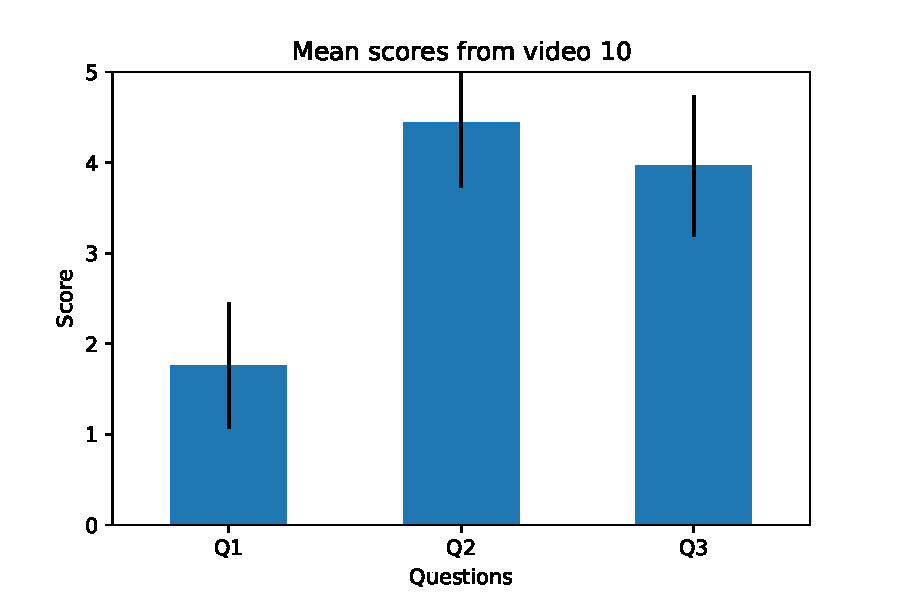
\includegraphics[width=0.6\textwidth]{img/subjective_measures/analysis/video_10.pdf}
    \caption{Subjective rating on video 10}
    \label{fig:visual_subj_vid10}
\end{figure}

\begin{table}[H]
    \centering
    \begin{tabular}{|c|c c c|} 
        \hline
           & \textbf{Mean Score} & \textbf{Percentage of full score} & \textbf{Standard Deviation} \\ [0.5ex] 
        \hline
        Q1 & 1.759 & 35.185\% & 0.699 \\ [1ex] 
        Q2 & 4.444 & 88.889\% & 0.718 \\ [1ex] 
        Q3 & 3.963 & 79.259\% & 0.776 \\ [1ex] 
        \hline
    \end{tabular}
    \caption{Numerical metrics from subjective rating in video 10}
    \label{tab:numerical_subj_vid10}
\end{table}

%------------------------------------

%------------------------------------

\section{Video 11}
\subsection{Objective Measures}

\begin{minipage}[c]{0.475\textwidth}
\begin{table}[H]
    \centering
    \begin{tabular}{||c c c||} 
        \hline
        \acrshort{iou} & \acrshort{dc} & \acrshort{pa} \\ [0.5ex] 
        \hline\hline
        94.166\% & 96.995\% & 99.265\% \\ [1ex] 
        \hline
    \end{tabular}
    \caption{Average metrics}
    \label{tab:metrics_video_11}
\end{table}
\end{minipage}
\begin{minipage}[c]{0.475\textwidth}
\begin{table}[H]
    \centering
    \begin{tabular}{||c c c||} 
        \hline
        \acrshort{tp} & \acrshort{tn} & \acrshort{fpn} \\ [0.5ex] 
        \hline\hline
        245737 & 1812624 & 15239 \\ [1ex] 
        \hline
    \end{tabular}
    \caption{Average pixel classification}
    \label{tab:pixels_video_11}
\end{table}
\end{minipage}

\subsection{Subjective Measures}

\begin{figure}[H]
    \centering
    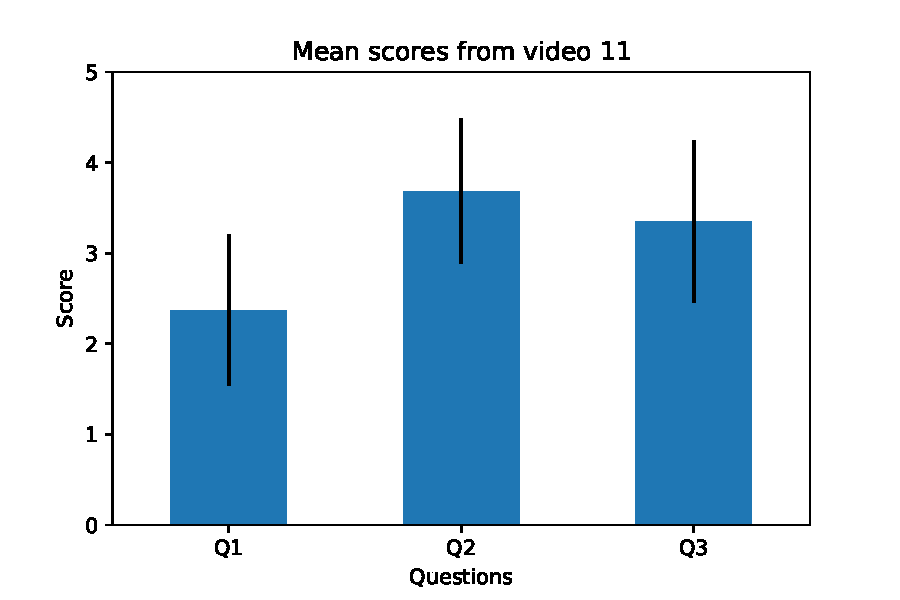
\includegraphics[width=0.6\textwidth]{img/subjective_measures/analysis/video_11.pdf}
    \caption{Subjective rating on video 11}
    \label{fig:visual_subj_vid11}
\end{figure}

\begin{table}[H]
    \centering
    \begin{tabular}{|c|c c c|} 
        \hline
           & \textbf{Mean Score} & \textbf{Percentage of full score} & \textbf{Standard Deviation} \\ [0.5ex] 
        \hline
        Q1 & 2.370 & 47.407\% & 0.831 \\ [1ex] 
        Q2 & 3.685 & 73.704\% & 0.797 \\ [1ex] 
        Q3 & 3.352 & 67.037\% & 0.894 \\ [1ex] 
        \hline
    \end{tabular}
    \caption{Numerical metrics from subjective rating in video 11}
    \label{tab:numerical_subj_vid11}
\end{table}


%------------------------------------

%------------------------------------

\section{Video 12}
\subsection{Objective Measures}

\begin{minipage}[c]{0.475\textwidth}
\begin{table}[H]
    \centering
    \begin{tabular}{||c c c||} 
        \hline
        \acrshort{iou} & \acrshort{dc} & \acrshort{pa} \\ [0.5ex] 
        \hline\hline
        93.845\% & 96.834\% & 99.220\% \\ [1ex] 
        \hline
    \end{tabular}
    \caption{Average metrics}
    \label{tab:metrics_video_12}
\end{table}
\end{minipage}
\begin{minipage}[c]{0.475\textwidth}
\begin{table}[H]
    \centering
    \begin{tabular}{||c c c||} 
        \hline
        \acrshort{tp} & \acrshort{tn} & \acrshort{fpn} \\ [0.5ex] 
        \hline\hline
        246300 & 181136 & 16164 \\ [1ex] 
        \hline
    \end{tabular}
    \caption{Average pixel classification}
    \label{tab:pixels_video_12}
\end{table}
\end{minipage}

\subsection{Subjective Measures}

\begin{figure}[H]
    \centering
    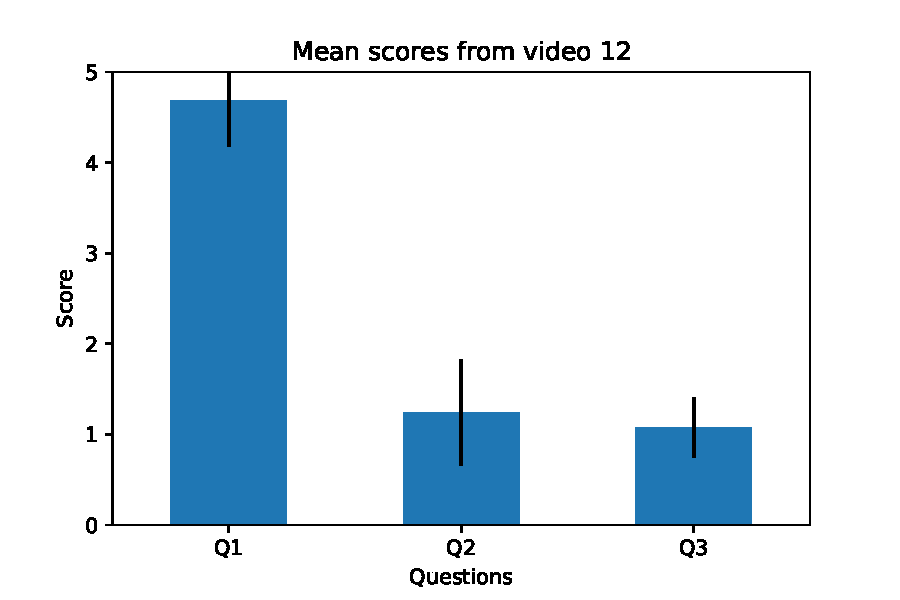
\includegraphics[width=0.6\textwidth]{img/subjective_measures/analysis/video_12.pdf}
    \caption{Subjective rating on video 12}
    \label{fig:visual_subj_vid12}
\end{figure}

\begin{table}[H]
    \centering
    \begin{tabular}{|c|c c c|} 
        \hline
           & \textbf{Mean Score} & \textbf{Percentage of full score} & \textbf{Standard Deviation} \\ [0.5ex] 
        \hline
        Q1 & 4.685 & 93.704\% & 0.507 \\ [1ex] 
        Q2 & 1.241 & 24.815\% & 0.581 \\ [1ex] 
        Q3 & 1.074 & 21.481\% & 0.328 \\ [1ex] 
        \hline
    \end{tabular}
    \caption{Numerical metrics from subjective rating in video 12}
    \label{tab:numerical_subj_vid12}
\end{table}


\subsection{Qualitative Feedback}
The participants were able to provide some additional feedback at the end of the questionnaire if they wanted to. The comments can be found in \autoref{cha:appendix-qualitative}.


%!TEX root = ../Thesis.tex
\chapter{Discussion}\label{cha:discussion}
%
\textcolor{red}{Here you should discuss all aspect of your thesis and project. How did the process work? Which choices did you make, and what did you learn from it? What were the pros and cons? What would you have done differently if you were to undertake the same project over again, both in terms of process and product? What are the societal consequences of your work?}

\section{Results}\label{sec:disc_results}
By studying the results from \autoref{cha:results} we see some interesting findings. A presentation of the results plotted with the video number on the x-axis can be found in \autoref{cha:appendix-video-rating}. Let's discuss some of our findings.

When we take a look at the first question of the subjective rating ("How satisfied are you with the quality of the silhouette extraction?") we see that video 4, 5 and 10 had the overall worst rating. The same applies for question 2 ("Did you notice any artefacts with the silhouette extraction?") and 3 ("Do you think the artefacts were annoying?")

We can also see that the three best videos from question 1, video 6, 9 and 12, also were the clear winners with the lowest level of noticeable artefacts and level of annoyance. While these videos were the clear winners from the subjective tests, it is not mirrored in the objective tests. 

Video 3 had the best objective score, but it was not popular in the subjective score. When we analyse this specific video closer we see what this might come from. This video has a few single bad frames with bad segmentation. While the objective scores does not penalise the single bad frames that much, it seems to be really annoying to watch for humans. Humans see these bad single frames as clear glitches and errors in the video. Some of the highest annoyance levels came from the videos with the best objective scores. 

The videos with the white wall performed overall better than all of the other backgrounds for the subjective measures, as expected (video 3, 6, 9 and 12). This is not the case for the objective measures, as there seems to be no clear pattern in which videos perform better than other. Sometimes the white wall background performed the best (video 3), and sometimes the window background performed the best (video 5 and 8).

Video 1, 2 and 3, where the person was showing an object, had almost the same rating for in the case of the subjective ratings. This was unrelated of the background. The results were not the worst either.

The levels of noticeable artefacts seems to be pretty linear with the level of annoyance for each video. There were no extreme cases where the participants thought the level of artefacts did not impact the perceived quality of the silhouette extraction.

We also notice something interesting with the dark and light clothing. The dark clothing, video 4, 5 and 6, got a overall much better rating objectively than the white clothing. But, when we look at the subjective rating, the light clothing got a much better score. One final interesting note, is that the dark and light clothing performed almost equally good objectively with the white wall background (video 5 and 8).

As far as we can see, there is no clear connection between the objective measures and the subjective measures, meaning none of our supporting hypothesis of our research questions were correct. The best subjectively rated videos, was overall not greatly rated objectively and vice versa.


\section{Quality of Experience}\label{sec:disc_qoe}

As already mentioned in \autoref{sec:previous} the measure of Quality of Experience can be a cumbersome task. Quality of Experience is by itself very subjective, up to each personal users viewpoint and relationship to whats in question. 

The perceived level of ''good quality'' varies in a large extent from person to person. We can ask ourselves what even is quality of experience? How would we be able to measure this in a way when each experience is so individual for each human being. 

There is no single scalar value which can be put to this. Only what we as human feel ourselves. The subjective rating results presented in this thesis has no definite answer, and it is up to each reader to evaluate with themselves if they think the results were sufficiently good enough to put the label of a high quality of experience on it. 


\section{The videos}\label{sec:disc_videos}

With the limited time frame and level of resources in such a thesis, only a selected number of test videos could be performed. By extending the number of videos to represent a larger number of use cases and variations, we could be able to get a more representative result on the level of quality of the \acrlong{mlbfe}. 

The constructed videos were constructed of foreground videos with a white male in his twenties representing a very small number of people which will be able to use this technology in the future. The different background videos were also constructed to represent some different challenges for the algorithm to work with, but they are not very representative of the final ''backgrounds'' that's going to be used in the field. One can imagine that the final users will more often than not film themselves in their living rooms, and not at a university campus. 

The videos did also not present other scenarios which one could imagine would be challenging. To name a few – Different types of lighting, picking up objects, more movement in the background, several people in the frame and outdoor filming. 

Another small thing to note, is that because of the green screen setup, we were unable to film a full body. This resulted in videos where the person had its feet cut off, and this might not be representative of the final use cases where most likely the entire bodies of the in frame persons will be used. 

While the placement of the ring lights were decided by trial and error to minimise shadow casting, we saw that this could have been improved in the chroma-key editing. Some of the videos had some shading issues, leading to a not entirely perfect chroma-key deletion. This was accounted for by adjusting the settings, giving pretty decent results despite of the shadowing. The shadow casting might give us a wrong ground truth since the silhouette will be bigger and not perfectly covering only the body of the person in the frame. Because of this, it might happen that the \acrshort{mlbfe} will perform better than the chroma-keying, but the objective rating will be penalised since it will see the machine learning cutting too much of the silhouette. The shadowing problem could be solved with improved lighting, either by using more lights or use other lighting technique. 

\section{Subjective Testing}\label{sec:disc_subjective}

The subjective testing in this thesis was done using a web form run through Google Forms. This was done as the view was that it was more important to get a larger amount of data, than what would have been possible by a physical survey. As this thesis also was done the fall of 2021, the Corona pandemic was still a part of our every day, making it even harder to recruit people to do physical testing. By using Google Forms we made an easy and readily available survey that could easily be shared with a lot of people. Because of this we got a good number of participants for the survey. 

But doing the testing via a web survey also introduces a lot of new influencing factors. Since the form was sent directly to the participants, the participants were able to do the survey in an uncontrolled environment. System influencing factors and context influencing factors can play a huge role here. We have no way of knowing what type of device the participants were using. Some probably used their phones, some used their computers, all having different screen sizes and screen technology. This could influence the entire viewing experience and the total experience, 

Since the participant were able to do the questionnaire when and where they wanted, we do not how the context influencing factors affected them, such as location, time of day, interruption's and so on. 

The only possible way to put a video into the Google Forms, was to use Google's own video hosting service, YouTube. As mentioned in \autoref{sec:system_subjective} the videos were uploaded unlisted to a newly created account to minimise targeted recommendations and other pitfalls in the YouTube algorithm. Using simple YouTube videos, we have no way of controlling whether or not the participants saw the videos only once or multiple times. The participants could also have seen the video as is in the forms, watched it in full screen, watched the video in a new tab within YouTube's own website and therefore seen lots of other video suggestions. Again a lot of influencing factors which can have impacted the general experience of the user. 

The result may also be biased because of the demographic and human influencing factors. The vast majority of the participants were higher educated, and within the educated a majority of the science of technology. By looking at \autoref{fig:age}, one could argue the age was not very evenly distributed. The age group from 18 to 34 were highly represented, but the other groups had a varied representation. The age distribution from this testing might not be a good representation of the final user base of this technology. 

The order of how the videos would be presented was also randomised by a Python function. This was done to prevent the participants to see the same foreground videos after one another, but one could ponder if the order of the videos should be carefully selected or not. Maybe all of the same foregrounds, or the same backgrounds, should be presented after each other? Could this have given a completely different result?

\section{Subjective VS Objective}\label{sec:disc_qua}

We decided to try to measure both subjective and objective data for this thesis, as it was not given that only one of them would give a clear result on the actual quality of the \acrlong{mlbfe}. 

During EPFL's development, they used similar objective testing like we have done in this thesis, to evaluate the technology. But since the final product will be used by real humans, the objective testing would not be quite representative of the final user experience. That is why we decided to go for both types of evaluations, to ensure a more representative result to the end use case, and to see if the objective and quantitative measures could yield a result with a matching pattern for the subjective and qualitative testing.

In our final inspection of the result, it seems like we are unable to find any particular pattern between the objective measures, \acrshort{iou}, \acrshort{dc} and \acrshort{pa}, and the subjective measures of satisfaction, level of artefacts and level of annoyance in the \acrlong{mlbfe}, as discussed in \autoref{sec:disc_results}. This further enhances our claim of needing both the objective and the subjective measures. The objective measures might work better for evaluating the quality at a single frame level, while the subjective measures might work better for the evaluation of the entire video itself. 

The objective measures gives us an image of how each single frame gets segmented, but the average result of this measure, does not give a clear result. To better utilise the objective measures, one should use an another way of presenting the final result than the average, as the extremes gets crushed by the other good performing frames. 

The subjective measures reflects the extremes clearer as the videos with single bad frames spread in the video got a bad rating. The single sporadic bad frames, of an otherwise good segmented video, impacted the participants quality of experience in a more profound way than the videos with smaller extremes, but overall might have had a weaker objective score. 

To combat this, the machine learning model could maybe implement ways to get rid of the extremes. For example – In the testing used in this thesis, the extremes were single bad frames. These single bad frames could maybe be digitally manipulated to match the surrounding frames. In video 3, where the person held a book, frame 256, seen in \autoref{fig:256}, had a \acrlong{fpn} score of $20505$, while the previous frame, seen in \autoref{fig:255}, had $12723$, and the following frame, seen in \autoref{fig:256}, had $13071$. If the machine learning model had done an automatic content aware filling for the missing book in frame 256, the subjective measure might have suffered less, as the seemingly glitch would have been less prominent

\begin{figure}
\centering
\begin{subfigure}{.3\textwidth}
  \centering
  
\includegraphics[width=\linewidth]{img/256/FG_Showing-Object_BG_White-Wall_fg_255.jpg}
  \caption{Frame 255 of video 3}
  \label{fig:255}
\end{subfigure}%
\begin{subfigure}{.3\textwidth}
  \centering
  
\includegraphics[width=\linewidth]{img/256/FG_Showing-Object_BG_White-Wall_fg_256.jpg}
  \caption{Frame 256 of video 3}
  \label{fig:256}
\end{subfigure}%
\begin{subfigure}{.3\textwidth}
  \centering
  
\includegraphics[width=\linewidth]{img/256/FG_Showing-Object_BG_White-Wall_fg_257.jpg}
  \caption{Frame 257 of video 3}
  \label{fig:257}
\end{subfigure}
\caption{Show case of a single bad frame}
\label{fig:single_bad_frame}
\end{figure}

Another interesting note, also discussed a bit in \autoref{sec:disc_results}, was the difference in results of the dark and light clothing. This further highlights the different outcomes of the objective and subjective measures, where the dark clothing got a better rating objectively than the white, but the subjective rating yielded a better score for the light clothing. By manually comparing the dark clothing videos to the light clothing videos, there seems to be little difference between them. It could be interesting to see how the results would turn out if the background colour was a different colour than black. With the black clothing, it could maybe be difficult to distinguish the silhouette from the background. Maybe if the background was for example a typical bright green screen green, it would have yielded different results subjectively, since the silhouette could possibly be easier to separate from the background. 

\section{Data set}\label{sec:disc_data}
The \acrlong{mlbfe} model has been trained with the data set from \cite{gmnu21}, further elaborated in \autoref{sec:training}, and while this is a general data set for separating human silhouettes in the foreground from what ever background, one can wonder if this data set representing a wide enough data set preparing the model for all of the final use cases. 

In our testing, we specifically saw that the current model with its training struggled a bit with foreign objects in the foreground scene. Like with other machine learning models, it is often not the technology itself which is the weakness, but the amount of data which the model has been trained and validated on. To increase the performance, an increased size of the data set used for training might be beneficiary. 

%!TEX root = ../Thesis.tex
\chapter{Conclusion}\label{cha:conclusion}
%

\textcolor{red}{The conclusion chapter is usually quite short – a paragraph or two – mainly summarising what was achieved in the project. It should answer the \emph{claim} part of the introduction. It should also say something about what comes next (`future work').}

\printbibliography[heading=bibintoc,title={References}]

\appendix
%!TEX root = ../Thesis.tex
\chapter{GitHub Repository}\label{cha:appendix-github}
In the following GitHub repository, you can find all relevant documentation, files and material for the project. It also contains the result analysis with the questionnaire answers in the form of a CSV file, which then was analyzed using a Jupyter Notebook. The Notebook can be found in the repository as well. Additionally can all of the raw numerical data from the objective analysis be found here. The repository also contains a wiki with more casual notes that have been made throughout the project period leading up to this final report, along with more lively media showing off the experimental application (video/GIFs). 

\begin{displayquote}
    \large \textbf{https://github.com/petrepa/TFE4940}
\end{displayquote}

%\chapter{Pre-Testing Questionnaire}\label{cha:appendix-pre-testing}
%\includepdf[pages=-]{Questionnaires/pre_testing_questionnaire.pdf}

%\chapter{Post-Testing Questionnaire}\label{cha:appendix-post-testing}
%\includepdf[pages=-]{Questionnaires/post_testing_questionnaire.pdf}

\chapter{Backgrounds used in video}\label{cha:appendix-backgrounds}
\begin{figure}[H]
    \centering
    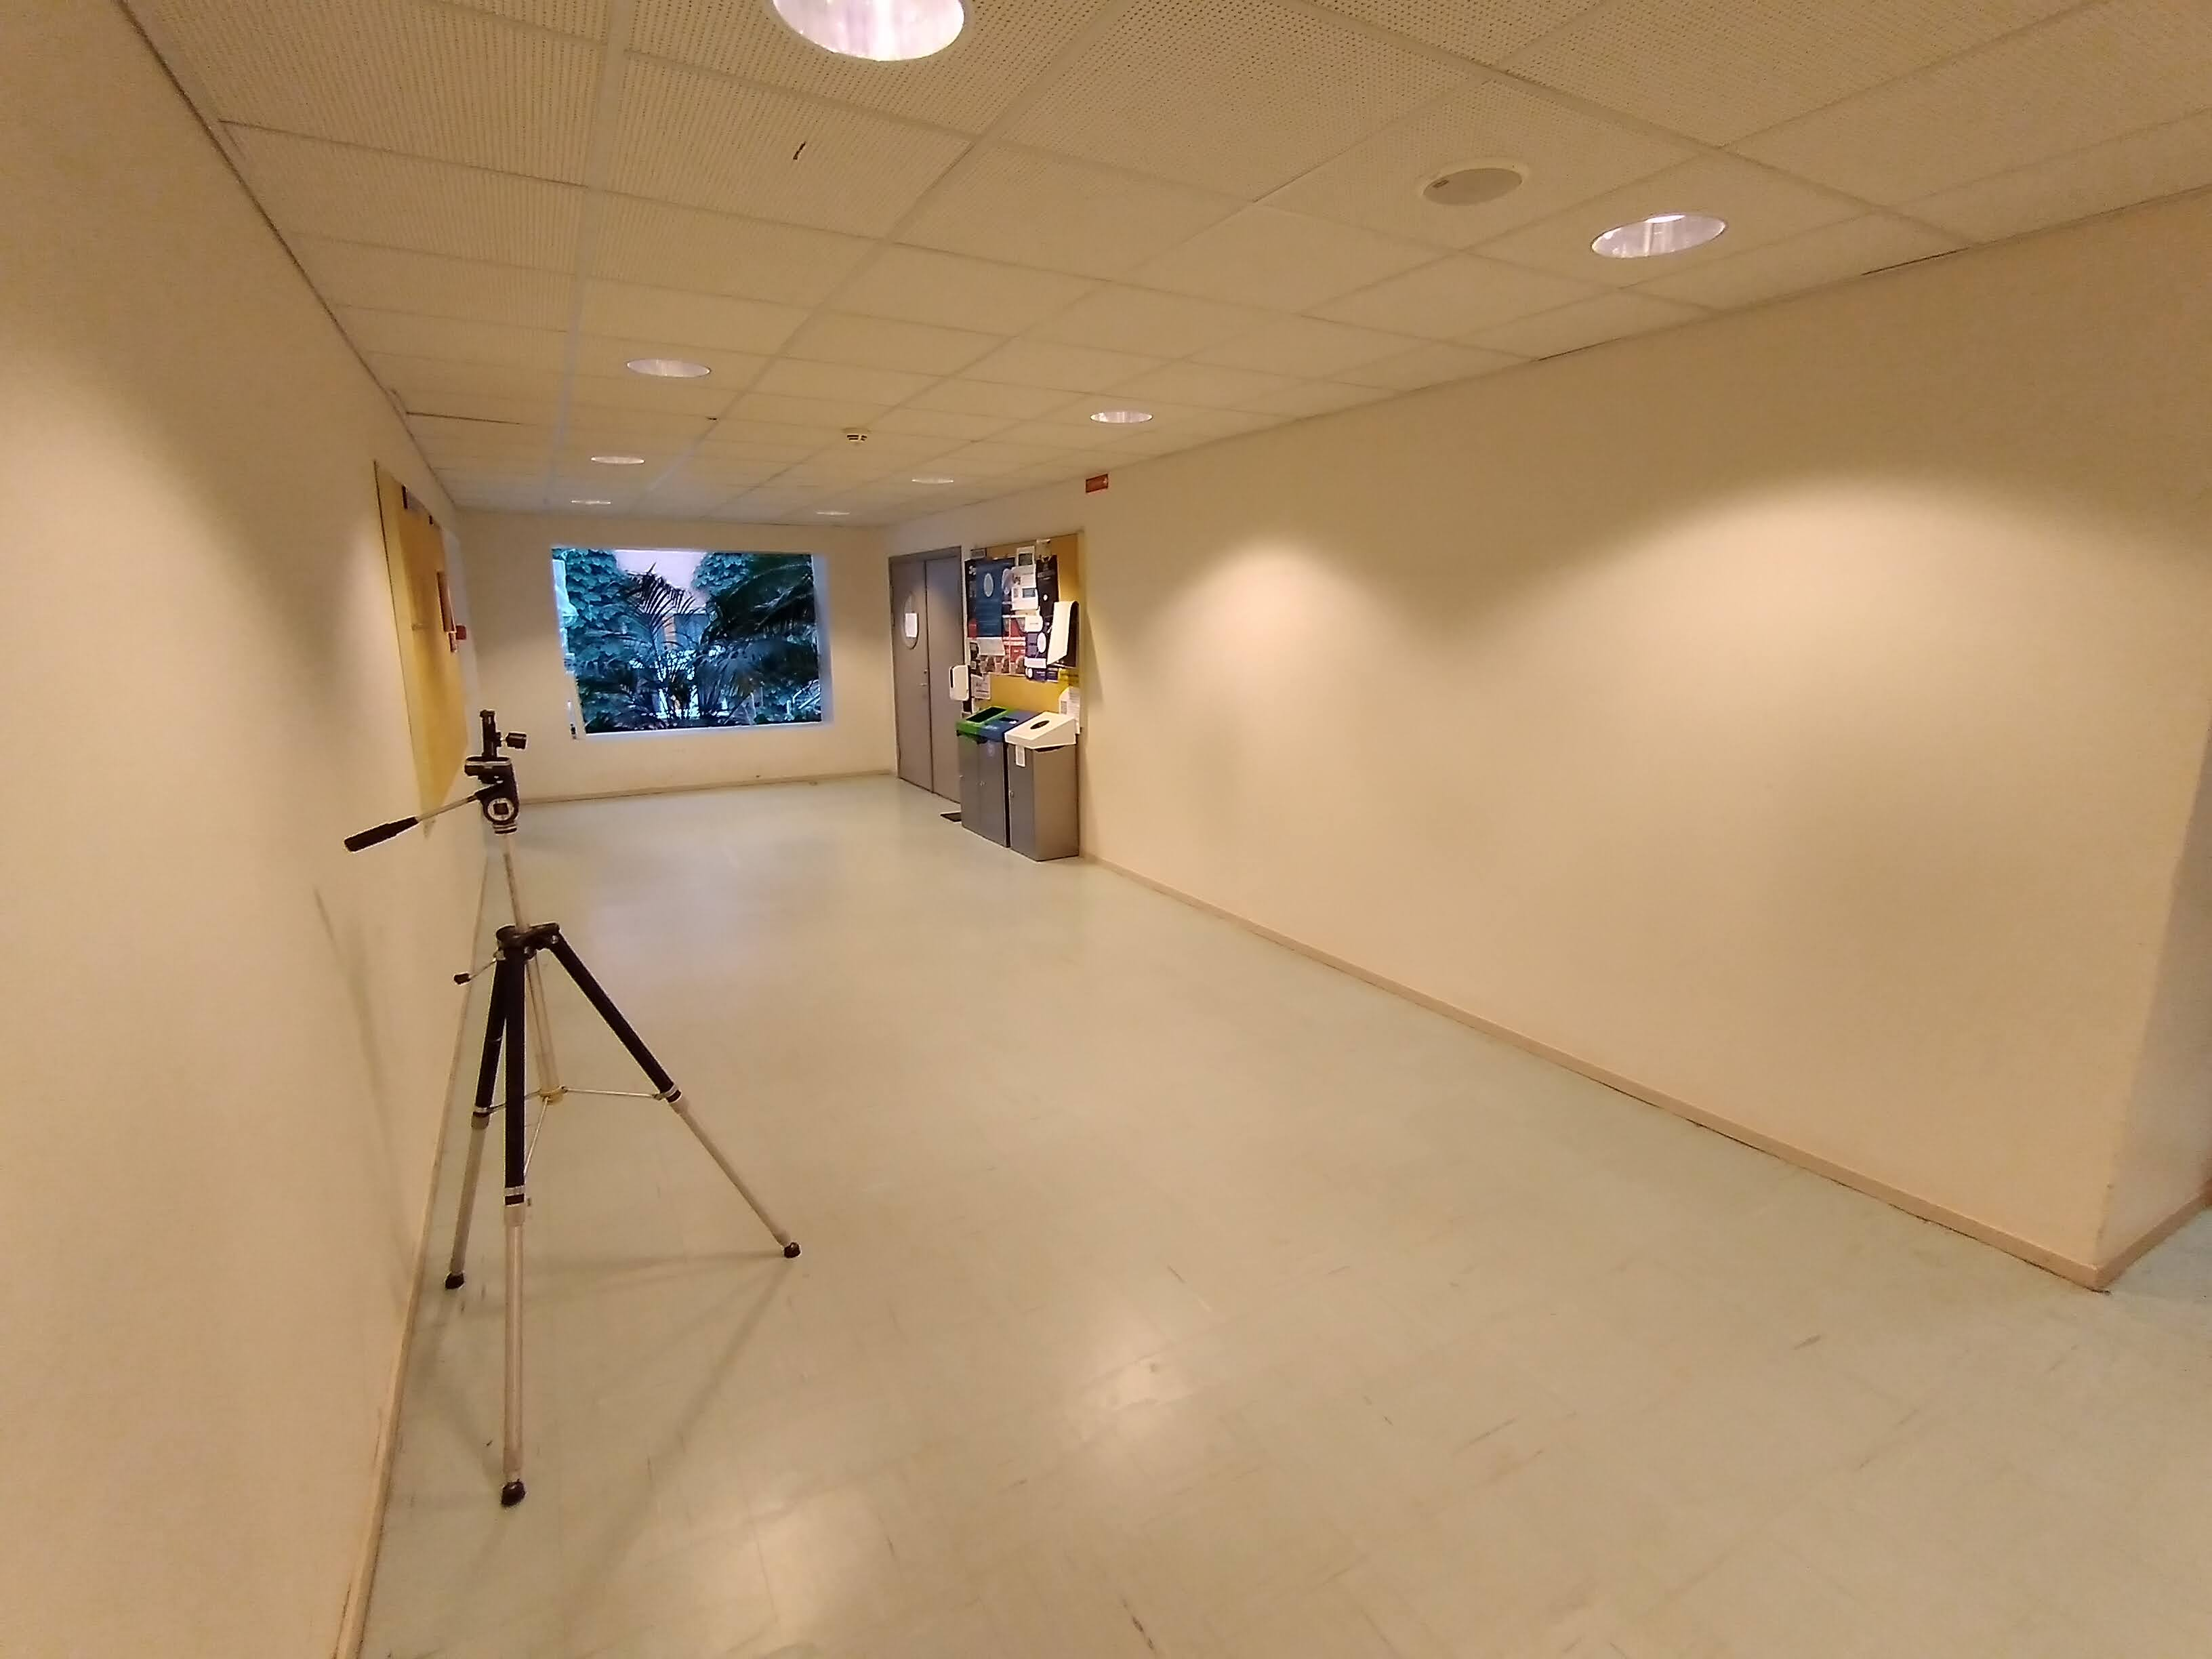
\includegraphics[width=\textwidth]{img/background_setup/simple_white_wall.jpg}
    \caption{Simple white wall}
    \label{fig:white_wall_setup}
\end{figure}
\begin{figure}[H]
    \centering
    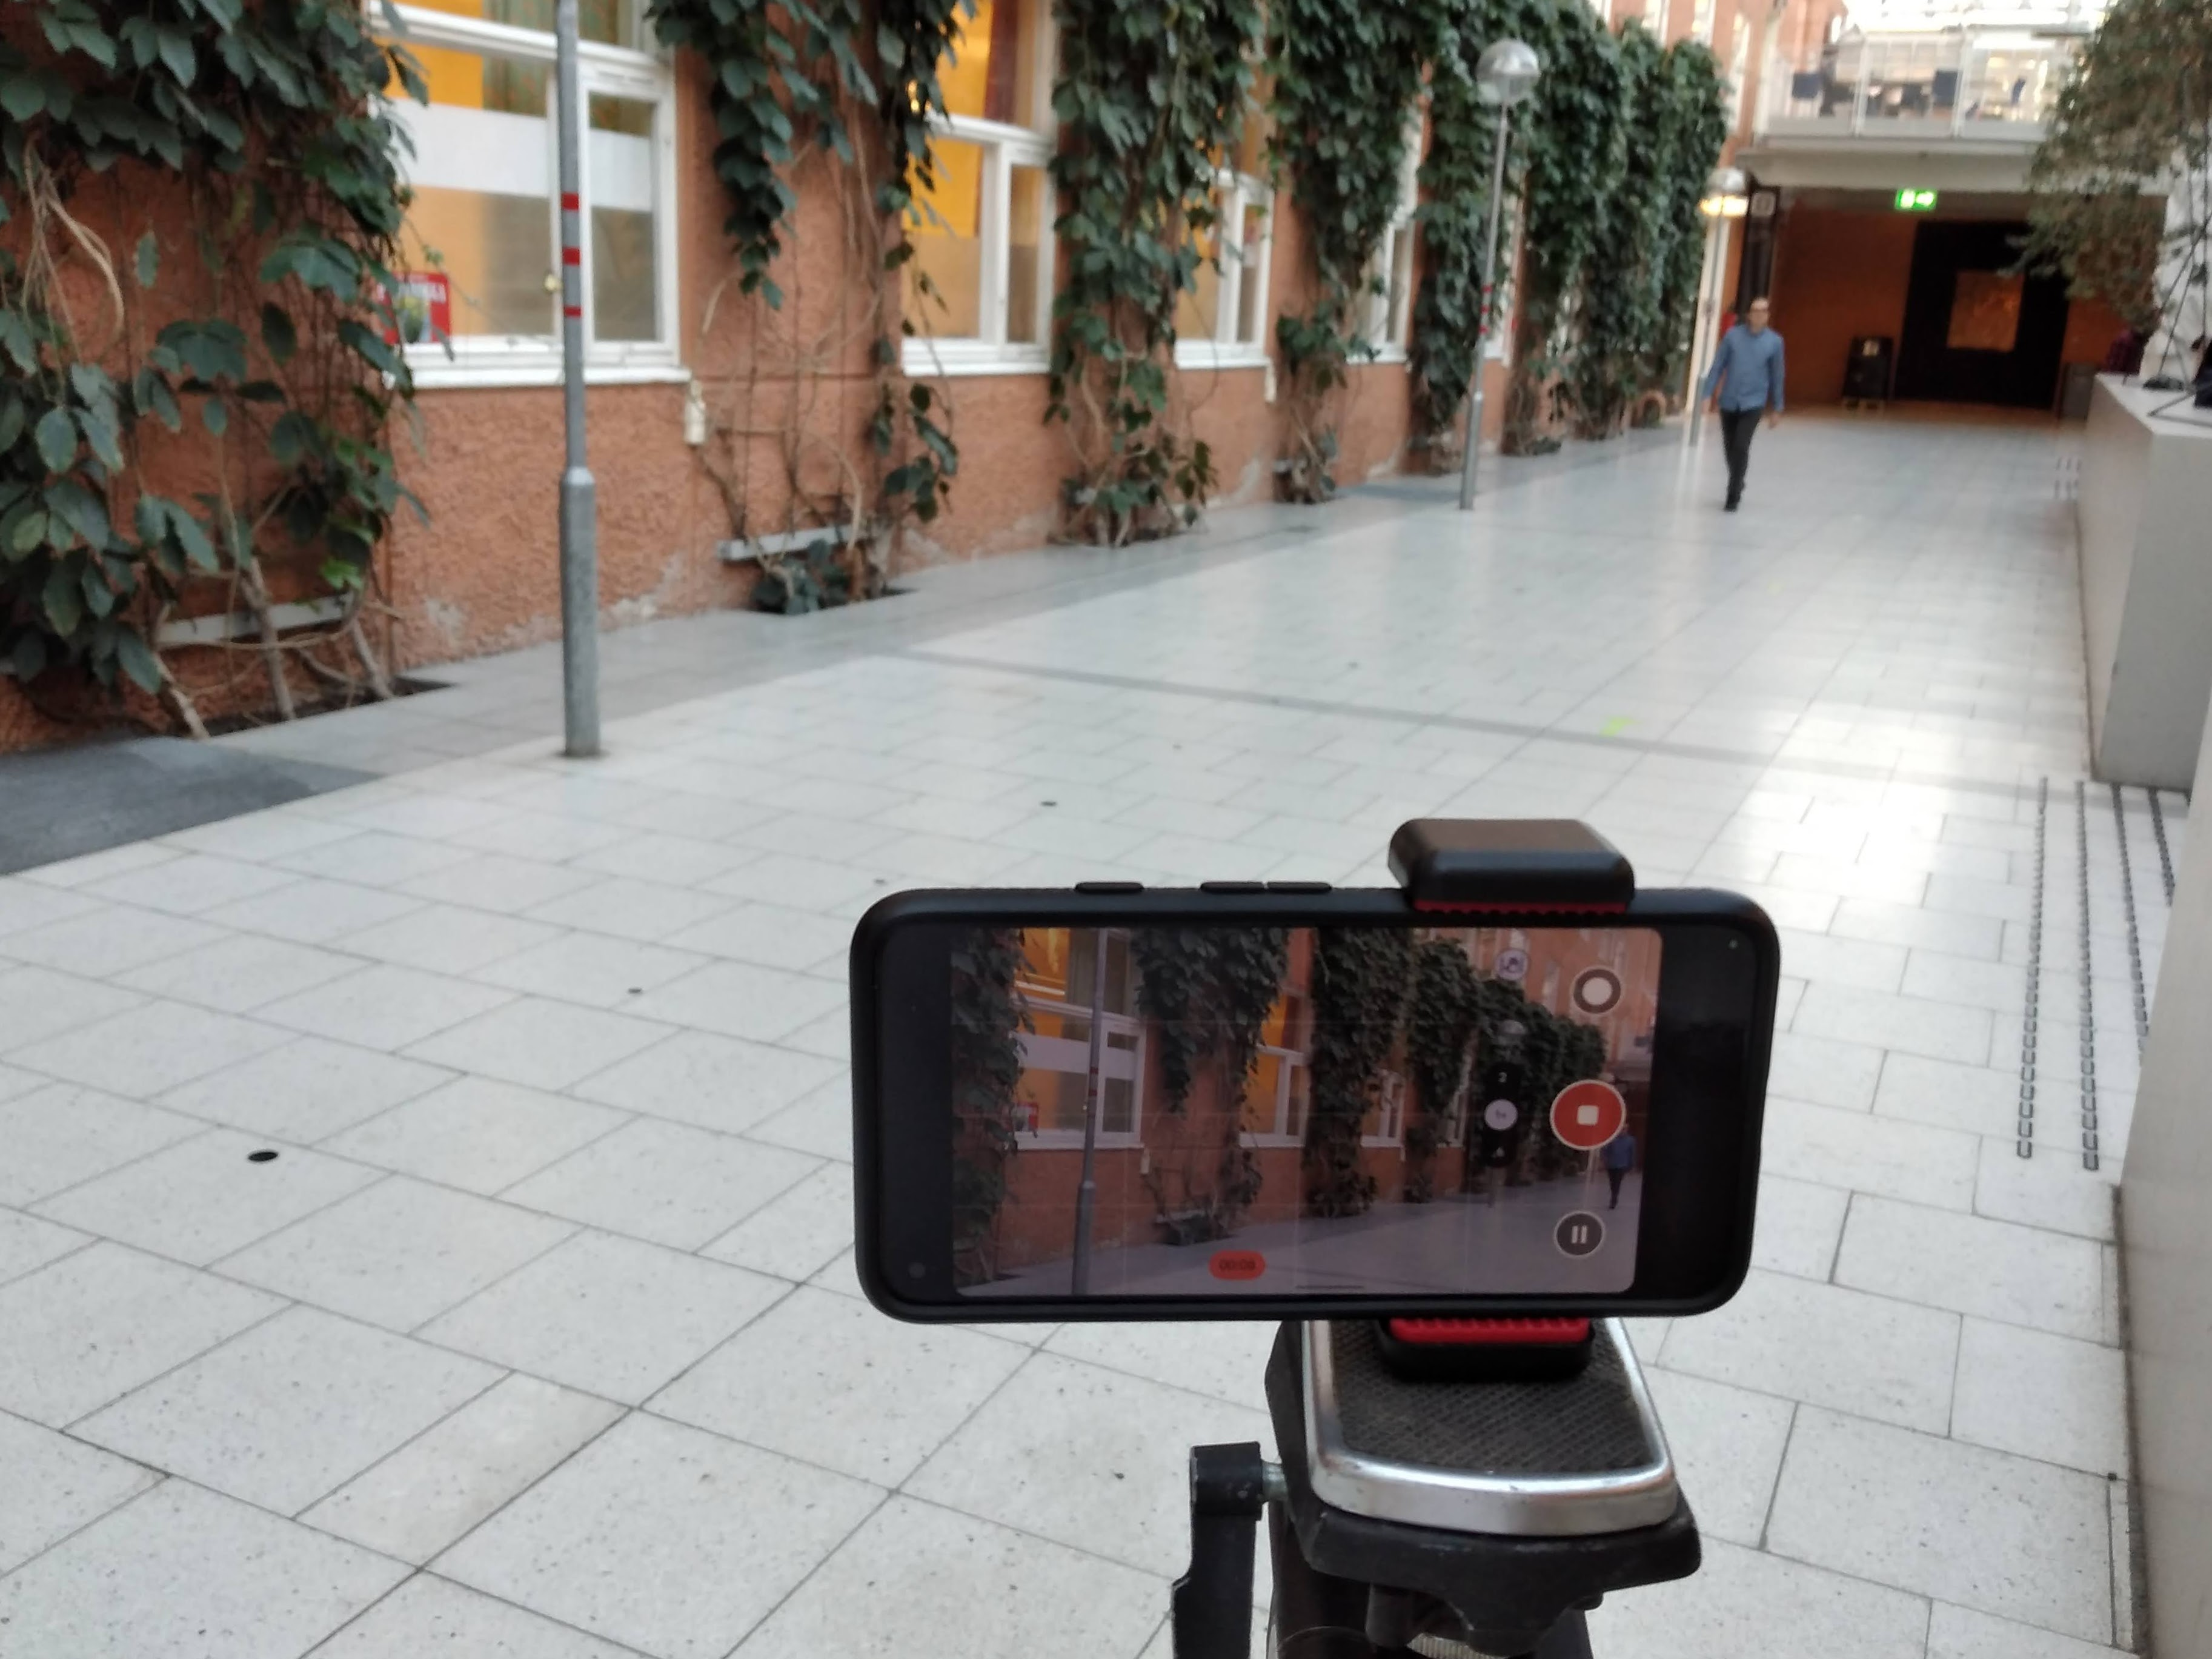
\includegraphics[width=\textwidth]{img/background_setup/complex_wall.jpg}
    \caption{Complex wall with different colors and textures}
    \label{fig:complex_setup}
\end{figure}
\begin{figure}[H]
    \centering
    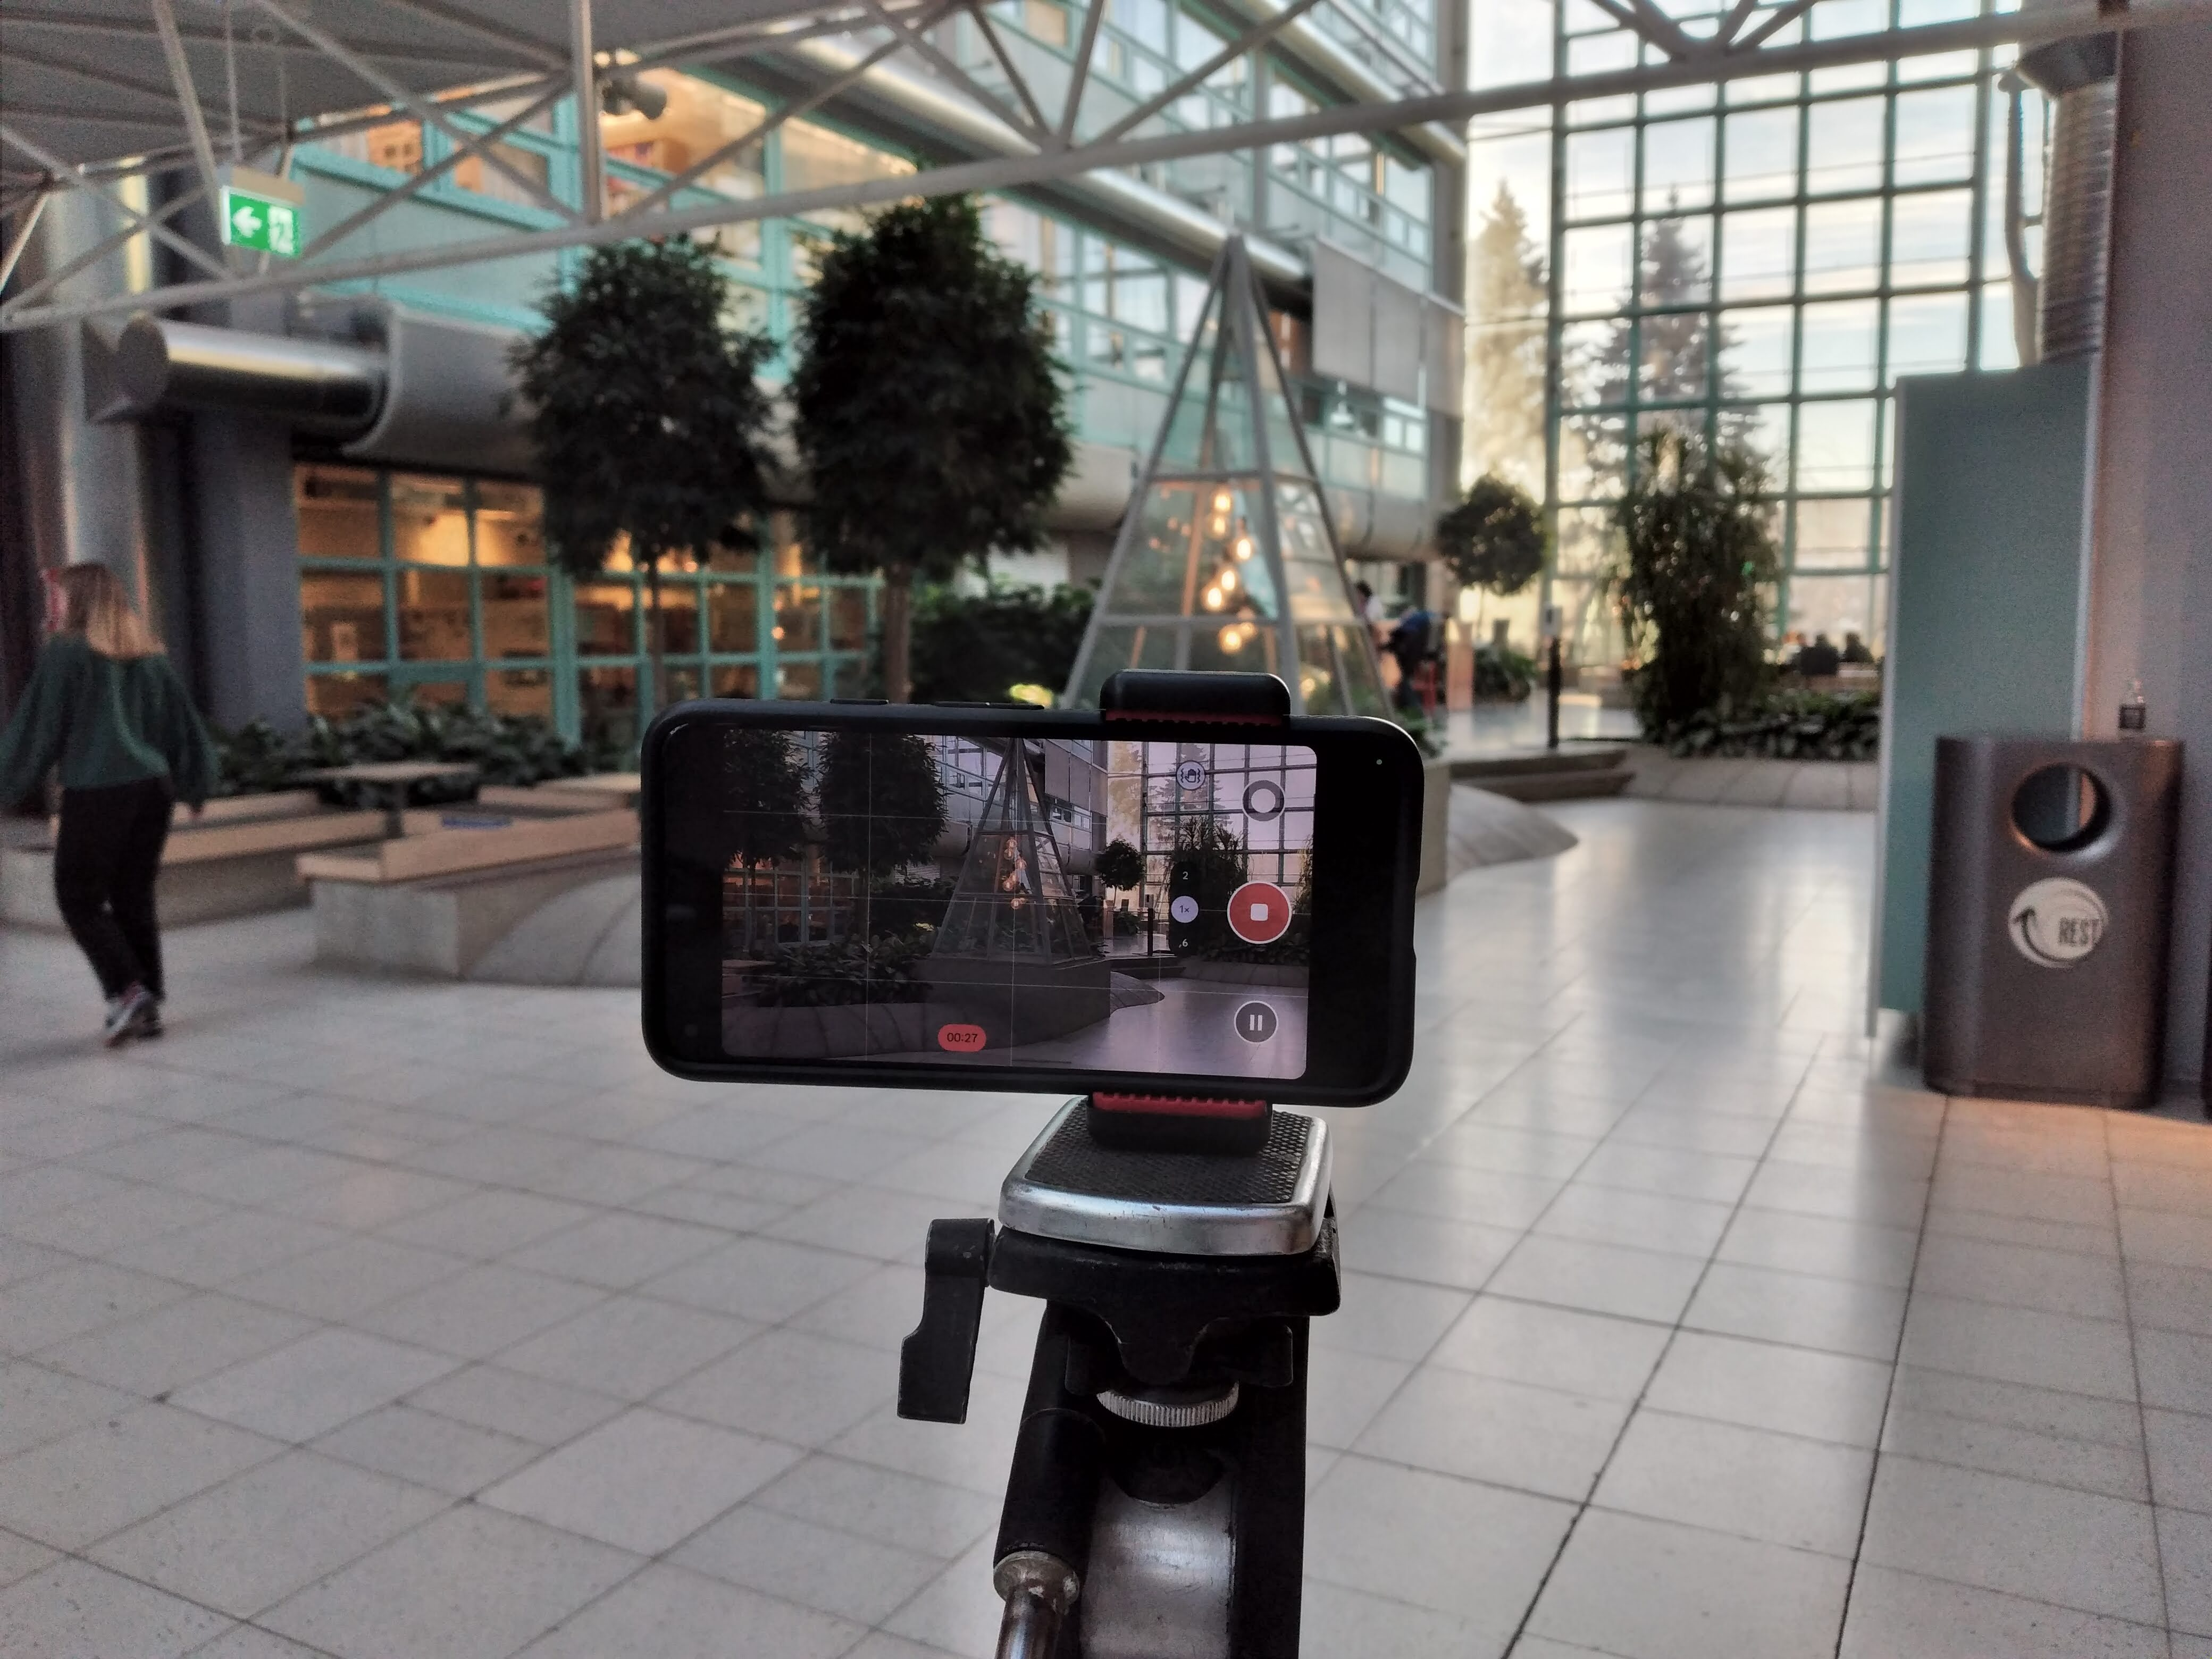
\includegraphics[width=\textwidth]{img/background_setup/windows.jpg}
    \caption{Background  with  windows  to  test for exposure difference and possible movements}
    \label{fig:windows_setup}
\end{figure}


\chapter{Questionnaire}\label{cha:appendix-questionnaire}
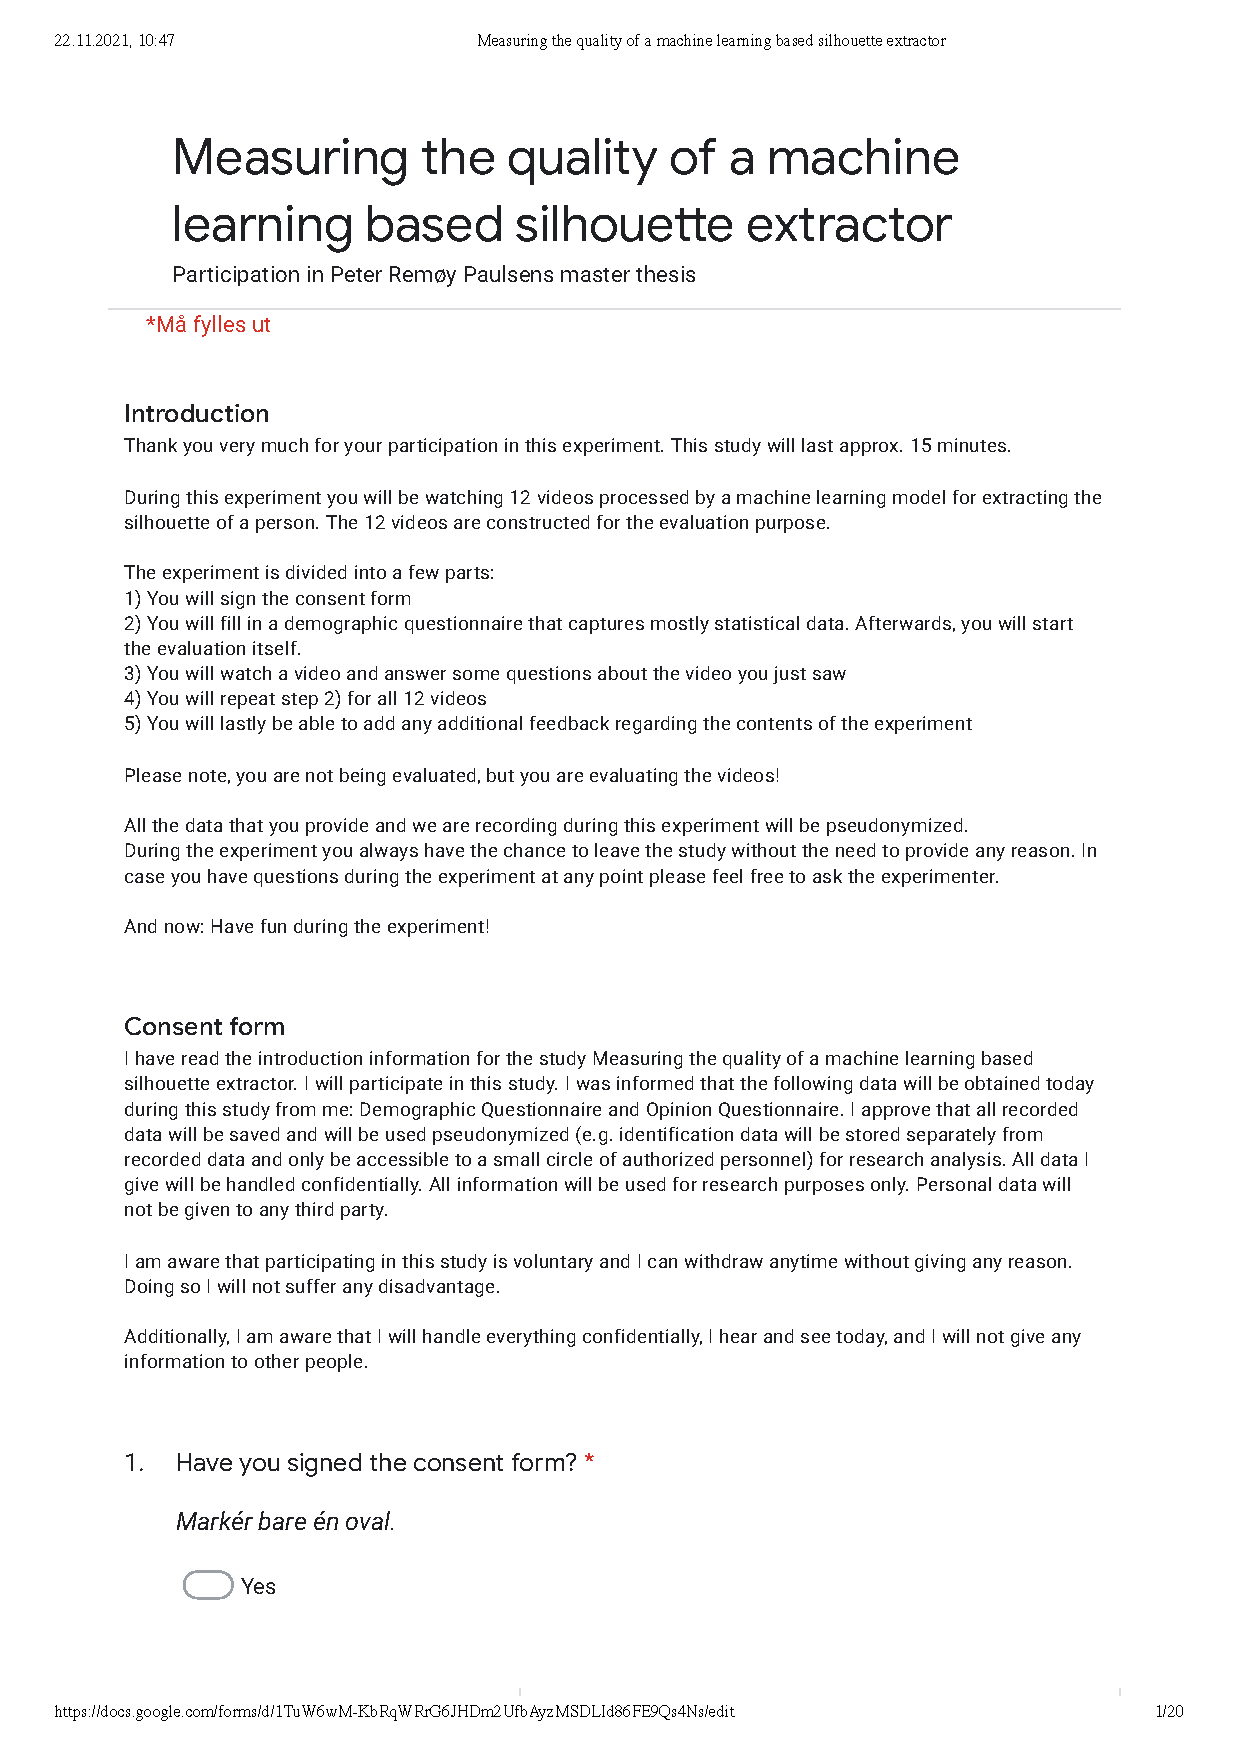
\includepdf[pages=-]{Questionnaires/Questionnaire.pdf}

\chapter{Videos}\label{cha:appendix-videos}
Here you can find the 150th frame of each video in both combined, \acrshort{mlbfe} processed, chroma key composition and black and white \acrshort{mlbfe} processed view.
\newpage
\section{Video 1}
\begin{figure}[H]
    \centering
        \begin{subfigure}[b]{0.475\textwidth}
            \centering
            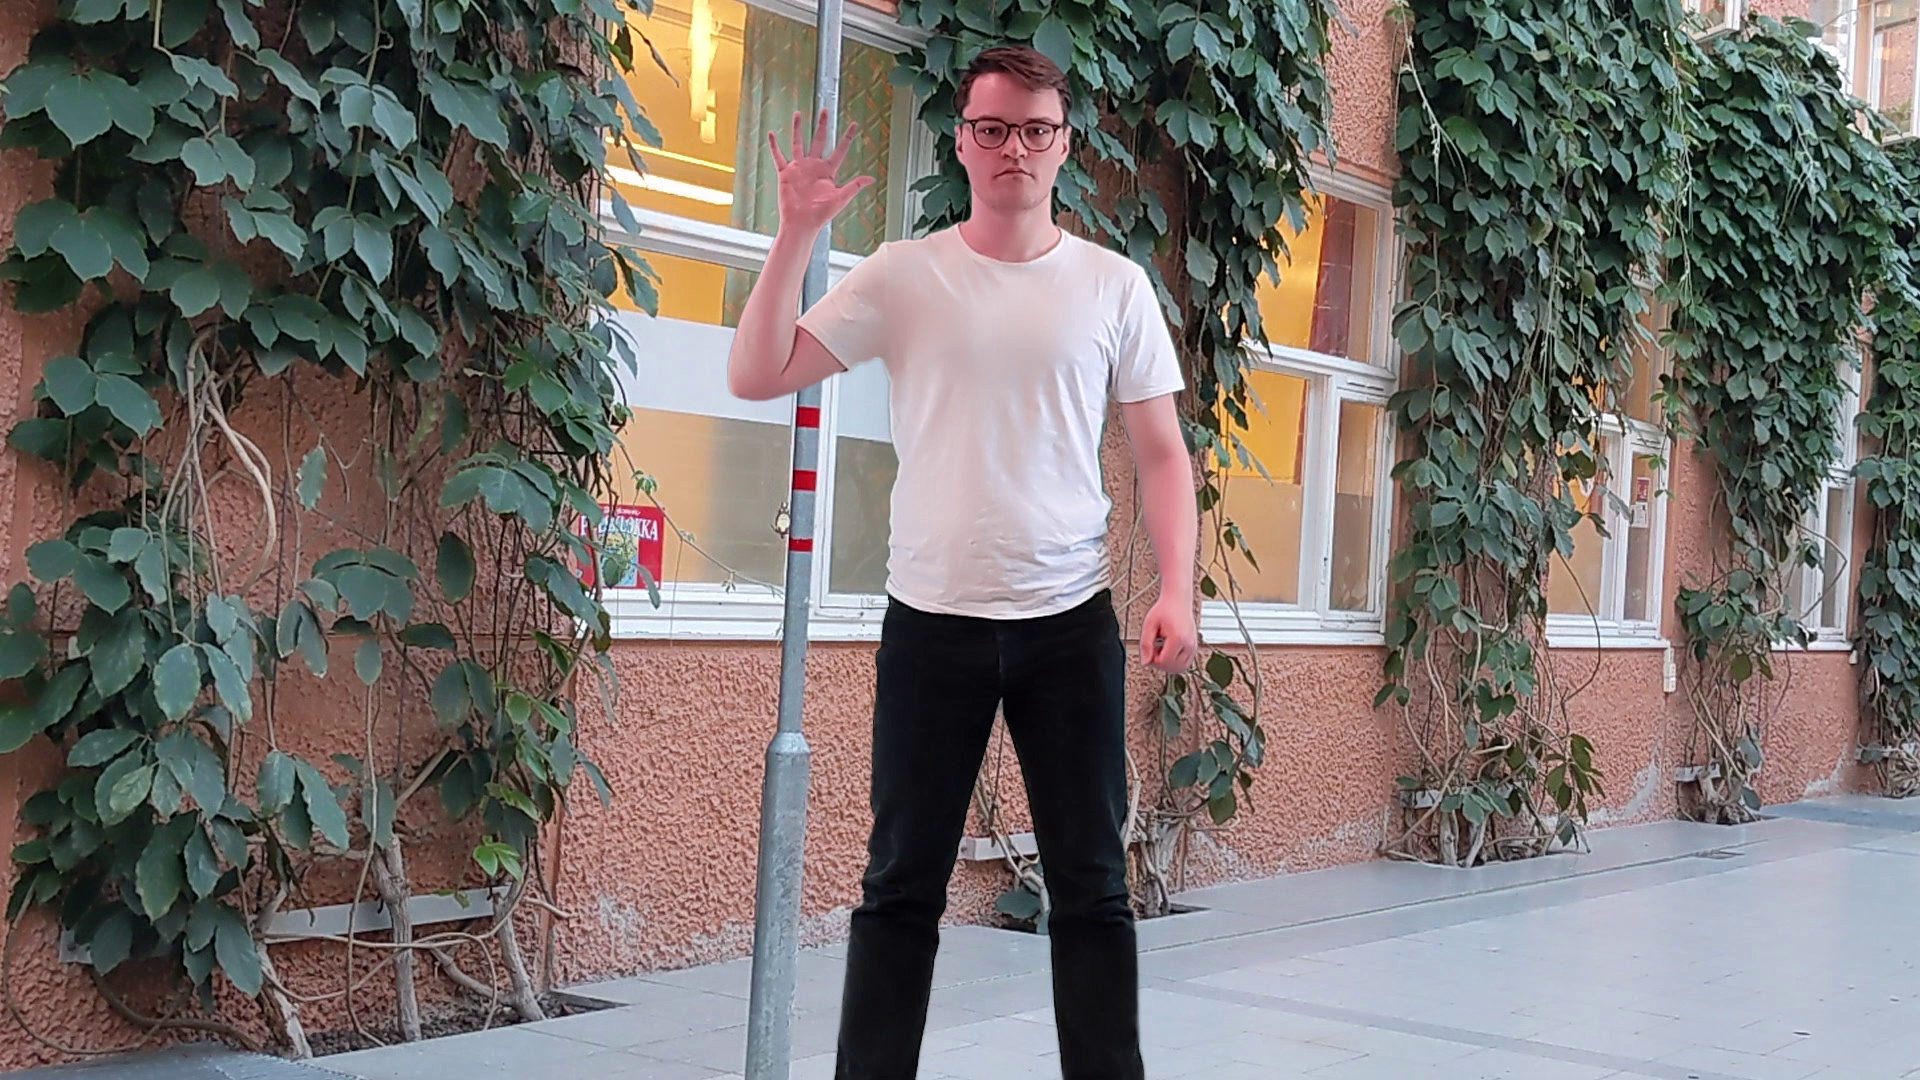
\includegraphics[width=\textwidth]{img/video_results/combined/FG_Counting-Fingers_BG_Complex_150.jpg}
            \caption[]%
            {{\small Foreground and background combined}}    
            \label{fig:video_1_combined}
        \end{subfigure}
    \hfill
        \begin{subfigure}[b]{0.475\textwidth}  
            \centering 
            
\includegraphics[width=\textwidth]{img/video_results/processed/FG_Counting-Fingers_BG_Complex_150.jpg}
            \caption[]%
            {{\small \acrshort{mlbfe} processed}}    
            \label{fig:video_1_processed}
        \end{subfigure}
    \vskip\baselineskip
        \begin{subfigure}[b]{0.475\textwidth}   
            \centering 
            
\includegraphics[width=\textwidth]{img/video_results/foreground_matte/FG_Counting-Fingers_150.jpg}
            \caption[]%
            {{\small Chroma Key Composition}}    
            \label{fig:video_1_matte}
        \end{subfigure}
    \hfill
        \begin{subfigure}[b]{0.475\textwidth}   
            \centering 
            
\includegraphics[width=\textwidth]{img/video_results/processed_BW/FG_Counting-Fingers_BG_Window_fg_150.jpg}
            \caption[]%
            {{\small Black \& white of \acrshort{mlbfe} processed}}    
            \label{fig:video_1_processed_BW}
        \end{subfigure}
    \caption[ Frame 150 from video 1 ]
    {\small Frame 150 from video 1} 
    \label{fig:frame_150_video_1}
\end{figure}


\section{Video 2}
\begin{figure}[H]
    \centering
        \begin{subfigure}[b]{0.475\textwidth}
            \centering
            
\includegraphics[width=\textwidth]{img/video_results/combined/FG_Counting-Fingers_BG_Window_150.jpg}
            \caption[]%
            {{\small Foreground and background combined}}    
            \label{fig:video_2_combined}
        \end{subfigure}
    \hfill
        \begin{subfigure}[b]{0.475\textwidth}  
            \centering 
            
\includegraphics[width=\textwidth]{img/video_results/processed/FG_Counting-Fingers_BG_Window_150.jpg}
            \caption[]%
            {{\small \acrshort{mlbfe} processed}}    
            \label{fig:video_2_processed}
        \end{subfigure}
    \vskip\baselineskip
        \begin{subfigure}[b]{0.475\textwidth}   
            \centering 
            
\includegraphics[width=\textwidth]{img/video_results/foreground_matte/FG_Counting-Fingers_150.jpg}
            \caption[]%
            {{\small Chroma Key Composition}}    
            \label{fig:video_2_matte}
        \end{subfigure}
    \hfill
        \begin{subfigure}[b]{0.475\textwidth}   
            \centering 
            
\includegraphics[width=\textwidth]{img/video_results/processed_BW/FG_Counting-Fingers_BG_Window_fg_150.jpg}
            \caption[]%
            {{\small Black \& white of \acrshort{mlbfe} processed}}    
            \label{fig:video_2_processed_BW}
        \end{subfigure}
    \caption[ Frame 150 from video 2 ]
    {\small Frame 150 from video 2} 
    \label{fig:frame_150_video_2}
\end{figure}


\section{Video 3}
\begin{figure}[H]
    \centering
        \begin{subfigure}[b]{0.475\textwidth}
            \centering
            
\includegraphics[width=\textwidth]{img/video_results/combined/FG_Counting-Fingers_BG_White-Wall_150.jpg}
            \caption[]%
            {{\small Foreground and background combined}}    
            \label{fig:video_3_combined}
        \end{subfigure}
    \hfill
        \begin{subfigure}[b]{0.475\textwidth}  
            \centering 
            \includegraphics[width=\textwidth]{img/video_results/processed/FG_Counting-Fingers_BG_White-Wall_150.jpg}
            \caption[]%
            {{\small \acrshort{mlbfe} processed}}    
            \label{fig:video_3_processed}
        \end{subfigure}
    \vskip\baselineskip
        \begin{subfigure}[b]{0.475\textwidth}   
            \centering 
            \includegraphics[width=\textwidth]{img/video_results/foreground_matte/FG_Counting-Fingers_150.jpg}
            \caption[]%
            {{\small Chroma Key Composition}}    
            \label{fig:video_3_matte}
        \end{subfigure}
    \hfill
        \begin{subfigure}[b]{0.475\textwidth}   
            \centering 
            \includegraphics[width=\textwidth]{img/video_results/processed_BW/FG_Counting-Fingers_BG_Window_fg_150.jpg}
            \caption[]%
            {{\small Black \& white of \acrshort{mlbfe} processed}}    
            \label{fig:video_3_processed_BW}
        \end{subfigure}
    \caption[ Frame 150 from video 3 ]
    {\small Frame 150 from video 3} 
    \label{fig:frame_150_video_3}
\end{figure}

\section{Video 4}
\begin{figure}[H]
    \centering
        \begin{subfigure}[b]{0.475\textwidth}
            \centering
            \includegraphics[width=\textwidth]{img/video_results/combined/FG_Rocking-Dark_BG_Complex_150.jpg}
            \caption[]%
            {{\small Foreground and background combined}}    
            \label{fig:video_4_combined}
        \end{subfigure}
    \hfill
        \begin{subfigure}[b]{0.475\textwidth}  
            \centering 
            \includegraphics[width=\textwidth]{img/video_results/processed/FG_Rocking-Dark_BG_Complex_150.jpg}
            \caption[]%
            {{\small \acrshort{mlbfe} processed}}    
            \label{fig:video_4_processed}
        \end{subfigure}
    \vskip\baselineskip
        \begin{subfigure}[b]{0.475\textwidth}   
            \centering 
            \includegraphics[width=\textwidth]{img/video_results/foreground_matte/FG_Rocking-Dark_150.jpg}
            \caption[]%
            {{\small Chroma Key Composition}}    
            \label{fig:video_4_matte}
        \end{subfigure}
    \hfill
        \begin{subfigure}[b]{0.475\textwidth}   
            \centering 
            \includegraphics[width=\textwidth]{img/video_results/processed_BW/FG_Rocking-Dark_BG_Complex_fg_150.jpg}
            \caption[]%
            {{\small Black \& white of \acrshort{mlbfe} processed}}    
            \label{fig:video_4_processed_BW}
        \end{subfigure}
    \caption[ Frame 150 from video 4 ]
    {\small Frame 150 from video 4} 
    \label{fig:frame_150_video_4}
\end{figure}

\section{Video 5}
\begin{figure}[H]
    \centering
        \begin{subfigure}[b]{0.475\textwidth}
            \centering
            \includegraphics[width=\textwidth]{img/video_results/combined/FG_Rocking-Dark_BG_Window_150.jpg}
            \caption[]%
            {{\small Foreground and background combined}}    
            \label{fig:video_5_combined}
        \end{subfigure}
    \hfill
        \begin{subfigure}[b]{0.475\textwidth}  
            \centering 
            \includegraphics[width=\textwidth]{img/video_results/processed/FG_Rocking-Dark_BG_Window_150.jpg}
            \caption[]%
            {{\small \acrshort{mlbfe} processed}}    
            \label{fig:video_5_processed}
        \end{subfigure}
    \vskip\baselineskip
        \begin{subfigure}[b]{0.475\textwidth}   
            \centering 
            \includegraphics[width=\textwidth]{img/video_results/foreground_matte/FG_Rocking-Dark_150.jpg}
            \caption[]%
            {{\small Chroma Key Composition}}    
            \label{fig:video_5_matte}
        \end{subfigure}
    \hfill
        \begin{subfigure}[b]{0.475\textwidth}   
            \centering 
            \includegraphics[width=\textwidth]{img/video_results/processed_BW/FG_Rocking-Dark_BG_Window_fg_150.jpg}
            \caption[]%
            {{\small Black \& white of \acrshort{mlbfe} processed}}    
            \label{fig:video_5_processed_BW}
        \end{subfigure}
    \caption[ Frame 150 from video 5 ]
    {\small Frame 150 from video 5} 
    \label{fig:frame_150_video_5}
\end{figure}

\section{Video 6}
\begin{figure}[H]
    \centering
        \begin{subfigure}[b]{0.475\textwidth}
            \centering
            \includegraphics[width=\textwidth]{img/video_results/combined/FG_Rocking-Dark_BG_White-Wall_150.jpg}
            \caption[]%
            {{\small Foreground and background combined}}    
            \label{fig:video_6_combined}
        \end{subfigure}
    \hfill
        \begin{subfigure}[b]{0.475\textwidth}  
            \centering 
            \includegraphics[width=\textwidth]{img/video_results/processed/FG_Rocking-Dark_BG_White-Wall_150.jpg}
            \caption[]%
            {{\small \acrshort{mlbfe} processed}}    
            \label{fig:video_6_processed}
        \end{subfigure}
    \vskip\baselineskip
        \begin{subfigure}[b]{0.475\textwidth}   
            \centering 
            \includegraphics[width=\textwidth]{img/video_results/foreground_matte/FG_Rocking-Dark_150.jpg}
            \caption[]%
            {{\small Chroma Key Composition}}    
            \label{fig:video_6_matte}
        \end{subfigure}
    \hfill
        \begin{subfigure}[b]{0.475\textwidth}   
            \centering 
            \includegraphics[width=\textwidth]{img/video_results/processed_BW/FG_Rocking-Dark_BG_White-Wall_fg_150.jpg}
            \caption[]%
            {{\small Black \& white of \acrshort{mlbfe} processed}}    
            \label{fig:video_6_processed_BW}
        \end{subfigure}
    \caption[ Frame 150 from video 6 ]
    {\small Frame 150 from video 6} 
    \label{fig:frame_150_video_7}
\end{figure}

\section{Video 7}
\begin{figure}[H]
    \centering
        \begin{subfigure}[b]{0.475\textwidth}
            \centering
            \includegraphics[width=\textwidth]{img/video_results/combined/FG_Rocking-Light_BG_Complex_150.jpg}
            \caption[]%
            {{\small Foreground and background combined}}    
            \label{fig:video_7_combined}
        \end{subfigure}
    \hfill
        \begin{subfigure}[b]{0.475\textwidth}  
            \centering 
            \includegraphics[width=\textwidth]{img/video_results/processed/FG_Rocking-Light_BG_Complex_150.jpg}
            \caption[]%
            {{\small \acrshort{mlbfe} processed}}    
            \label{fig:video_7_processed}
        \end{subfigure}
    \vskip\baselineskip
        \begin{subfigure}[b]{0.475\textwidth}   
            \centering 
            \includegraphics[width=\textwidth]{img/video_results/foreground_matte/FG_Rocking-Light_150.jpg}
            \caption[]%
            {{\small Chroma Key Composition}}    
            \label{fig:video_7_matte}
        \end{subfigure}
    \hfill
        \begin{subfigure}[b]{0.475\textwidth}   
            \centering 
            \includegraphics[width=\textwidth]{img/video_results/processed_BW/FG_Rocking-Light_BG_Complex_fg_150.jpg}
            \caption[]%
            {{\small Black \& white of \acrshort{mlbfe} processed}}    
            \label{fig:video_7_processed_BW}
        \end{subfigure}
    \caption[ Frame 150 from video 7 ]
    {\small Frame 150 from video 7} 
    \label{fig:frame_150_video_7}
\end{figure}

\section{Video 8}
\begin{figure}[H]
    \centering
        \begin{subfigure}[b]{0.475\textwidth}
            \centering
            \includegraphics[width=\textwidth]{img/video_results/combined/FG_Rocking-Light_BG_Window_150.jpg}
            \caption[]%
            {{\small Foreground and background combined}}    
            \label{fig:video_8_combined}
        \end{subfigure}
    \hfill
        \begin{subfigure}[b]{0.475\textwidth}  
            \centering 
            \includegraphics[width=\textwidth]{img/video_results/processed/FG_Rocking-Light_BG_Window_150.jpg}
            \caption[]%
            {{\small \acrshort{mlbfe} processed}}    
            \label{fig:video_8_processed}
        \end{subfigure}
    \vskip\baselineskip
        \begin{subfigure}[b]{0.475\textwidth}   
            \centering 
            \includegraphics[width=\textwidth]{img/video_results/foreground_matte/FG_Rocking-Light_150.jpg}
            \caption[]%
            {{\small Chroma Key Composition}}    
            \label{fig:video_8_matte}
        \end{subfigure}
    \hfill
        \begin{subfigure}[b]{0.475\textwidth}   
            \centering 
            \includegraphics[width=\textwidth]{img/video_results/processed_BW/FG_Rocking-Light_BG_Window_fg_150.jpg}
            \caption[]%
            {{\small Black \& white of \acrshort{mlbfe} processed}}    
            \label{fig:video_8_processed_BW}
        \end{subfigure}
    \caption[ Frame 150 from video 8 ]
    {\small Frame 150 from video 8} 
    \label{fig:frame_150_video_8}
\end{figure}

\section{Video 9}
\begin{figure}[H]
    \centering
        \begin{subfigure}[b]{0.475\textwidth}
            \centering
            \includegraphics[width=\textwidth]{img/video_results/combined/FG_Rocking-Light_BG_White-Wall_150.jpg}
            \caption[]%
            {{\small Foreground and background combined}}    
            \label{fig:video_9_combined}
        \end{subfigure}
    \hfill
        \begin{subfigure}[b]{0.475\textwidth}  
            \centering 
            \includegraphics[width=\textwidth]{img/video_results/processed/FG_Rocking-Light_BG_White-Wall_150.jpg}
            \caption[]%
            {{\small \acrshort{mlbfe} processed}}    
            \label{fig:video_9_processed}
        \end{subfigure}
    \vskip\baselineskip
        \begin{subfigure}[b]{0.475\textwidth}   
            \centering 
            \includegraphics[width=\textwidth]{img/video_results/foreground_matte/FG_Rocking-Light_150.jpg}
            \caption[]%
            {{\small Chroma Key Composition}}    
            \label{fig:video_9_matte}
        \end{subfigure}
    \hfill
        \begin{subfigure}[b]{0.475\textwidth}   
            \centering 
            \includegraphics[width=\textwidth]{img/video_results/processed_BW/FG_Rocking-Light_BG_White-Wall_fg_150.jpg}
            \caption[]%
            {{\small Black \& white of \acrshort{mlbfe} processed}}    
            \label{fig:video_9_processed_BW}
        \end{subfigure}
    \caption[ Frame 150 from video 9 ]
    {\small Frame 150 from video 9} 
    \label{fig:frame_150_video_9}
\end{figure}


\section{Video 10}
\begin{figure}[H]
    \centering
        \begin{subfigure}[b]{0.475\textwidth}
            \centering
            \includegraphics[width=\textwidth]{img/video_results/combined/FG_Counting-Fingers_BG_Complex_150.jpg}
            \caption[]%
            {{\small Foreground and background combined}}    
            \label{fig:video_10_combined}
        \end{subfigure}
    \hfill
        \begin{subfigure}[b]{0.475\textwidth}  
            \centering 
            \includegraphics[width=\textwidth]{img/video_results/processed/FG_Counting-Fingers_BG_Complex_150.jpg}
            \caption[]%
            {{\small \acrshort{mlbfe} processed}}    
            \label{fig:video_10_processed}
        \end{subfigure}
    \vskip\baselineskip
        \begin{subfigure}[b]{0.475\textwidth}   
            \centering 
            \includegraphics[width=\textwidth]{img/video_results/foreground_matte/FG_Counting-Fingers_150.jpg}
            \caption[]%
            {{\small Chroma Key Composition}}    
            \label{fig:video_10_matte}
        \end{subfigure}
    \hfill
        \begin{subfigure}[b]{0.475\textwidth}   
            \centering 
            \includegraphics[width=\textwidth]{img/video_results/processed_BW/FG_Counting-Fingers_BG_Complex_fg_150.jpg}
            \caption[]%
            {{\small Black \& white of \acrshort{mlbfe} processed}}    
            \label{fig:video_10_processed_BW}
        \end{subfigure}
    \caption[ Frame 150 from video 10 ]
    {\small Frame 150 from video 10} 
    \label{fig:frame_150_video_10}
\end{figure}

\section{Video 11}
\begin{figure}[H]
    \centering
        \begin{subfigure}[b]{0.475\textwidth}
            \centering
            \includegraphics[width=\textwidth]{img/video_results/combined/FG_Counting-Fingers_BG_Window_150.jpg}
            \caption[]%
            {{\small Foreground and background combined}}    
            \label{fig:video_11_combined}
        \end{subfigure}
    \hfill
        \begin{subfigure}[b]{0.475\textwidth}  
            \centering 
            \includegraphics[width=\textwidth]{img/video_results/processed/FG_Counting-Fingers_BG_Window_150.jpg}
            \caption[]%
            {{\small \acrshort{mlbfe} processed}}    
            \label{fig:video_11_processed}
        \end{subfigure}
    \vskip\baselineskip
        \begin{subfigure}[b]{0.475\textwidth}   
            \centering 
            \includegraphics[width=\textwidth]{img/video_results/foreground_matte/FG_Counting-Fingers_150.jpg}
            \caption[]%
            {{\small Chroma Key Composition}}    
            \label{fig:video_11_matte}
        \end{subfigure}
    \hfill
        \begin{subfigure}[b]{0.475\textwidth}   
            \centering 
            \includegraphics[width=\textwidth]{img/video_results/processed_BW/FG_Counting-Fingers_BG_Window_fg_150.jpg}
            \caption[]%
            {{\small Black \& white of \acrshort{mlbfe} processed}}    
            \label{fig:video_11_processed_BW}
        \end{subfigure}
    \caption[ Frame 150 from video 11 ]
    {\small Frame 150 from video 11} 
    \label{fig:frame_150_video_11}
\end{figure}

\section{Video 12}
\begin{figure}[H]
    \centering
        \begin{subfigure}[b]{0.475\textwidth}
            \centering
            \includegraphics[width=\textwidth]{img/video_results/combined/FG_Counting-Fingers_BG_White-Wall_150.jpg}
            \caption[]%
            {{\small Foreground and background combined}}    
            \label{fig:video_12_combined}
        \end{subfigure}
    \hfill
        \begin{subfigure}[b]{0.475\textwidth}  
            \centering 
            \includegraphics[width=\textwidth]{img/video_results/processed/FG_Counting-Fingers_BG_White-Wall_150.jpg}
            \caption[]%
            {{\small \acrshort{mlbfe} processed}}    
            \label{fig:video_12_processed}
        \end{subfigure}
    \vskip\baselineskip
        \begin{subfigure}[b]{0.475\textwidth}   
            \centering 
            \includegraphics[width=\textwidth]{img/video_results/foreground_matte/FG_Counting-Fingers_150.jpg}
            \caption[]%
            {{\small Chroma Key Composition}}    
            \label{fig:video_12_matte}
        \end{subfigure}
    \hfill
        \begin{subfigure}[b]{0.475\textwidth}   
            \centering 
            \includegraphics[width=\textwidth]{img/video_results/processed_BW/FG_Counting-Fingers_BG_White-Wall_fg_150.jpg}
            \caption[]%
            {{\small Black \& white of \acrshort{mlbfe} processed}}    
            \label{fig:video_12_processed_BW}
        \end{subfigure}
    \caption[ Frame 150 from video 12 ]
    {\small Frame 150 from video 12} 
    \label{fig:frame_150_video_12}
\end{figure}
\chapter{Qualitative Feedback}\label{cha:appendix-qualitative}


\begin{longtable}{p{0.5cm}p{11cm}}
\caption{Qualitative Feedback}
\label{tab:qualitative_feedback}\\
    \hline
        1 & The examples are good \\
        \hline
        2 & Likte dansen \\
        \hline
        3 & Undersøkelse med høg kvalitet.\\
        \hline
        4 & Vet ikke helt hva jeg svarte på her men du tar deg godt ut på video :) milla \\
        \hline
        5 & Imponerende teknologi. Ser at små detaljer er vanskeligere å trekke ut enn større. Eksperimentet med boken er også interessant. Siden denne er større en fingrene, burde det vært mindre klipping på den, men det kan ha med lys, farge og refleksjon i overflaten på boken. Uansett en veldig imponerende teknologi, da jeg regner med dette er gjort uten green-screen \\
        \hline
        6 & Generelt meir irriterande på dei videoane der bakgrunnen tidvis flimrar inn i bildet - veldig "visuelt" forstyrrande. Der det manglar ein finger eller to oppfattast som mindre irriterande, så lenge feilen "vedvarer" (ikkje blinkar/flimrar). Hjerna veit jo på ein måte at fingeren er der? PS. Masse lykke til med vidare arbeid med masteren! Hang in there :-)\\
        \hline
        7 & Det var mykje lik kvalitet på videoane. Eg var stort sett ikkje fornøgd med nåken av dei. \\
        \hline
        8 & Veldig bra! Mest minus til det som forsvinner, feks hvis man skal vise frem forsiden av en bok og den blir "filtrert bort". Ikke like farlig/annoying med litt artefacts som henger igjen etter bevegelse.\\
        \hline
        9 & usikker på om eg skjønte spørsmåla, men trur det :) \\
        \hline
        10 & Morsom undersøkelse, bra jobbet! Den eneste tilbakemeldingen jeg har er at spørsmålene kanskje var litt for tekniske og det derfor var litt vanskelig å være sikker på at man skjønte hva du spør om. En liten introtekst til hva det handler om kunne vært fint. Da kunne du også definert noen begreper så alle vet hva det blir stilt spørsmål om. Evt skrive spørsmålene litt mer sånn som man ville snakket til en 5-åring. Men jeg likte undersøkelsen godt, det var gøy! Lykke til videre :) \\
        \hline
        11 & Ser ut som silhuettene skildres greit ut på kroppen, men noe flimring rundt fingrer og armer. \\
        \hline
        12 & Sakna ein piruett eller to, elles flott jobba!\\
        \hline
        13 & Kult prosjekt, ønsker mer variasjon i dansemoves til neste gang.\\
        \hline
        14 & Dette var et arti eksperiment med godt gjennomført spørreskjema og gode svaralternativer. Lurte kun på om fargene på klærne burde vært den samme? \\
        \hline
        15 & Blinking er mest irriterende \\
        \hline
        16 & Svært interessant :D \\
        \hline
        17 & Nice presentation. Impressed our the video quality. \\
        \hline
        18 & Seems that in some videos the silhouette extractor works very well, but on what seems to be identical tests the extractor also struggles a lot, even when the object wears identical clothes. \\
        \hline
        19 & V beautiful videos. This could be an art exhibition<33 \\
        \hline
        20 & Interesting work! Looking forward to read the final thesis \\
        \hline
\end{longtable}

\backmatter
 
\end{document}
